











    \section{Discrete univariate with finite support}
        

        
    
        
\subsection{Zipf–Mandelbrot law}





% \begin{tabularx}{\textwidth}{l | X}
    {\color{darkblue} \textbf{Params.}:} {$N \in \{1,2,3\ldots\}$ (integer),  $q \in [0;\infty)$ (real),  $s>0\,$ (real)};\hspace{0.5cm}{\color{darkblue} \textbf{$\mathcal{W}(X)$}:} {$k \in \{1,2,\ldots,N\}$};\hspace{0.5cm}{\color{darkblue} \textbf{$\mathbb{E}[X]$}:} {$\frac{H_{N,q,s-1}}{H_{N,q,s}}-q$};\hspace{0.5cm}\\{\color{darkblue} \textbf{$f_x$}:} {$\frac{1/(k+q)^s}{H_{N,q,s}}$}{\color{darkblue} \textbf{$F_x$}:} {$\frac{H_{k,q,s}}{H_{N,q,s}}$}
% \end{tabularx}



    
        
\subsection{Poisson binomial distribution}





% \begin{tabularx}{\textwidth}{l | X}
    {\color{darkblue} \textbf{Params.}:} {$\mathbf{p}\in [0,1]^n$ — success probabilities for each of the \textit{n} trials};\hspace{0.5cm}{\color{darkblue} \textbf{$\mathcal{W}(X)$}:} {\textit{k} ∈ { 0, …, \textit{n} }};\hspace{0.5cm}{\color{darkblue} \textbf{$\mathbb{E}[X]$}:} {$\sum\limits_{i=1}^n p_i$};\hspace{0.5cm}{\color{darkblue} \textbf{$Var[X]$}:} {$ \sigma^2 =\sum\limits_{i=1}^n (1 - p_i)p_i$};\hspace{0.5cm}\\{\color{darkblue} \textbf{$f_x$}:} {$\sum\limits_{A\in F_k} \prod\limits_{i\in A} p_i \prod\limits_{j\in A^c} (1-p_j)$}{\color{darkblue} \textbf{$F_x$}:} {$\sum\limits_{l=0}^k \sum\limits_{A\in F_l} \prod\limits_{i\in A} p_i \prod\limits_{j\in A^c} (1-p_j)$}
% \end{tabularx}



    
        
\subsection{Rademacher distribution}





% \begin{tabularx}{\textwidth}{l | X}
    {\color{darkblue} \textbf{$\mathcal{W}(X)$}:} {$k \in \{-1,1\}\,$};\hspace{0.5cm}{\color{darkblue} \textbf{$\mathbb{E}[X]$}:} {$0\,$};\hspace{0.5cm}{\color{darkblue} \textbf{$Var[X]$}:} {$1\,$};\hspace{0.5cm}\\{\color{darkblue} \textbf{$f_x$}:} {$$f(k) = \left\{\begin{matrix} 1/2 & \mbox {if }k=-1, \\
1/2 & \mbox {if }k=+1, \\
0 & \mbox {otherwise.}\end{matrix}\right.$$}{\color{darkblue} \textbf{$F_x$}:} {$$F(k) = 
    \begin{cases}
     0,   & k < -1 \\
     1/2, & -1 \leq k < 1 \\
     1,   & k \geq 1
    \end{cases}$$}
% \end{tabularx}



    
        
\subsection{Bernoulli distribution}





% \begin{tabularx}{\textwidth}{l | X}
    {\color{darkblue} \textbf{Params.}:} {$0 \leq p \leq 1$ ,  $q = 1 - p$};\hspace{0.5cm}{\color{darkblue} \textbf{$\mathcal{W}(X)$}:} {$k \in \{0,1\}$};\hspace{0.5cm}{\color{darkblue} \textbf{$\mathbb{E}[X]$}:} {$ p$};\hspace{0.5cm}{\color{darkblue} \textbf{$Var[X]$}:} {$p(1-p) = pq $};\hspace{0.5cm}\\{\color{darkblue} \textbf{$f_x$}:} {$$\begin{cases}
    q=1-p & \text{if }k=0 \\
    p & \text{if }k=1
    \end{cases}$$}{\color{darkblue} \textbf{$F_x$}:} {$$\begin{cases}
    0 & \text{if } k < 0 \\
    1 - p & \text{if } 0 \leq k < 1 \\
    1 & \text{if } k \geq 1
    \end{cases}$$}
% \end{tabularx}



    
        
\subsection{Beta-binomial distribution}


    \begin{figure}[H]
        \centering
        \includegraphics[width=0.6\textwidth]{images/Beta-binomial distribution pmf.png}
        \caption{Probability mass function for the beta-binomial distribution}
    \end{figure}




% \begin{tabularx}{\textwidth}{l | X}
    {\color{darkblue} \textbf{Params.}:} {\textit{n} ∈ \textbf{N}\textsubscript{0} — number of trials,  $\alpha > 0$ (real) ,  $\beta > 0$ (real)};\hspace{0.5cm}{\color{darkblue} \textbf{$\mathcal{W}(X)$}:} {\textit{k} ∈ { 0, …, \textit{n} }};\hspace{0.5cm}{\color{darkblue} \textbf{$\mathbb{E}[X]$}:} {$\frac{n\alpha}{\alpha+\beta}\!$};\hspace{0.5cm}{\color{darkblue} \textbf{$Var[X]$}:} {$\frac{n\alpha\beta(\alpha+\beta+n)}{(\alpha+\beta)^2(\alpha+\beta+1)}\!$};\hspace{0.5cm}\\{\color{darkblue} \textbf{$f_x$}:} {$\binom{n}{k} \frac{\mathrm{B}(k+\alpha,n-k+\beta)} {\mathrm{B}(\alpha,\beta)}\!$}{\color{darkblue} \textbf{$F_x$}:} {$\begin{cases} 0,& k < 0 \\ \binom{n}{k} \tfrac{\mathrm{B}(k+\alpha,n-k+\beta)} {\mathrm{B}(\alpha,\beta)} {}_3\!F_2(\boldsymbol{a},\boldsymbol{b},k), & 0 \le k < n \\ 1,& k \geq n \end{cases}$ , , where <big> \textsubscript{3}\textit{F}\textsubscript{2}(\textbf{a},\textbf{b},k)</big> is the generalized hypergeometric function,  <small> ${}_3\!F_2(1, -k, n\! -\! k\! +\! \beta; n\! -\! k\! -\! 1, 1\! -\! k\! -\! \alpha; 1)\!$ </small>}
% \end{tabularx}



    
        
\subsection{Zipf's law}


    \begin{figure}[H]
        \centering
        \includegraphics[width=0.6\textwidth]{images/Zipf distribution PMF.png}
        \caption{Plot of the Zipf PMF for \textit{N} = 10}
    \end{figure}




% \begin{tabularx}{\textwidth}{l | X}
    {\color{darkblue} \textbf{Params.}:} {$s \geq 0\,$ (real),  $N \in \{1,2,3\ldots\}$ (integer)};\hspace{0.5cm}{\color{darkblue} \textbf{$\mathcal{W}(X)$}:} {$k \in \{1,2,\ldots,N\}$};\hspace{0.5cm}{\color{darkblue} \textbf{$\mathbb{E}[X]$}:} {$\frac{H_{N,s-1}}{H_{N,s}}$};\hspace{0.5cm}{\color{darkblue} \textbf{$Var[X]$}:} {$\frac{H_{N,s-2}}{H_{N,s}}-\frac{H^2_{N,s-1}}{H^2_{N,s}}$};\hspace{0.5cm}\\{\color{darkblue} \textbf{$f_x$}:} {$\frac{1/k^s}{H_{N,s}}$ where \textit{H\textsubscript{N,s}} is the \textit{N}th generalized harmonic number}{\color{darkblue} \textbf{$F_x$}:} {$\frac{H_{k,s}}{H_{N,s}}$}
% \end{tabularx}



    
        
\subsection{Binomial distribution}


    \begin{figure}[H]
        \centering
        \includegraphics[width=0.6\textwidth]{images/Binomial distribution pmf.png}
        \caption{Probability mass function for the binomial distribution}
    \end{figure}




% \begin{tabularx}{\textwidth}{l | X}
    {\color{darkblue} \textbf{Params.}:} {$n \in \{0, 1, 2, \ldots\}$ – number of trials,  $p \in [0,1]$ – success probability for each trial,  $q = 1 - p$};\hspace{0.5cm}{\color{darkblue} \textbf{Not.}:} {$B(n,p)$};\hspace{0.5cm}{\color{darkblue} \textbf{$\mathcal{W}(X)$}:} {$k \in \{0, 1, \ldots, n\}$ – number of successes};\hspace{0.5cm}{\color{darkblue} \textbf{$\mathbb{E}[X]$}:} {$np$};\hspace{0.5cm}{\color{darkblue} \textbf{$Var[X]$}:} {$npq$};\hspace{0.5cm}\\{\color{darkblue} \textbf{$f_x$}:} {$\binom{n}{k} p^k q^{n-k}$}{\color{darkblue} \textbf{$F_x$}:} {$I_{q}(n - k, 1 + k)$}
% \end{tabularx}



    
        
\subsection{Discrete uniform distribution}


    \begin{figure}[H]
        \centering
        \includegraphics[width=0.6\textwidth]{images/Uniform discrete pmf svg.png}
        \caption{Discrete uniform probability mass function for \textit{n} = 5}
    \end{figure}




% \begin{tabularx}{\textwidth}{l | X}
    {\color{darkblue} \textbf{Params.}:} {$a,b$ integers with $b \geq a$ ,  $n=b-a+1$};\hspace{0.5cm}{\color{darkblue} \textbf{Not.}:} {$\mathcal{U}\{a, b\}$ or $\mathrm{unif}\{a,b\}$};\hspace{0.5cm}{\color{darkblue} \textbf{$\mathcal{W}(X)$}:} {$k \in \{a,a+1,\dots,b-1,b\}$};\hspace{0.5cm}{\color{darkblue} \textbf{$\mathbb{E}[X]$}:} {$\frac{a+b}{2}$};\hspace{0.5cm}{\color{darkblue} \textbf{$Var[X]$}:} {$\frac{(b-a+1)^2-1}{12}$};\hspace{0.5cm}\\{\color{darkblue} \textbf{$f_x$}:} {$\frac{1}{n}$}{\color{darkblue} \textbf{$F_x$}:} {$ \frac{\lfloor k \rfloor -a+1}{n} $}
% \end{tabularx}



    


    \section{Discrete univariate with infinite support}
        

        
    
        
\subsection{Beta negative binomial distribution}





% \begin{tabularx}{\textwidth}{l | X}
    {\color{darkblue} \textbf{Params.}:} {$\alpha > 0$ shape (real),  $\beta > 0$ shape (real) ,  $r > 0$ — number of failures until the experiment is stopped (integer but can be extended to real)};\hspace{0.5cm}{\color{darkblue} \textbf{$\mathcal{W}(X)$}:} {\textit{k} ∈ { 0, 1, 2, 3, ... }};\hspace{0.5cm}{\color{darkblue} \textbf{$\mathbb{E}[X]$}:} {$$\begin{cases}
              \frac{r\beta}{\alpha-1} & \text{if}\ \alpha>1    \\
              \infty & \text{otherwise}\ \end{cases}$$};\hspace{0.5cm}{\color{darkblue} \textbf{$Var[X]$}:} {$$\begin{cases}
              \frac{r(\alpha+r-1)\beta(\alpha+\beta-1)}{(\alpha-2){(\alpha-1)}^2} & \text{if}\ \alpha>2    \\
              \infty & \text{otherwise}\ \end{cases}$$};\hspace{0.5cm}\\{\color{darkblue} \textbf{$f_x$}:} {$\frac{\Gamma(r+k)}{k!\;\Gamma(r)} \frac{\mathrm{B}(\alpha+r,\beta+k)} {\mathrm{B}(\alpha,\beta)}$}
% \end{tabularx}



    
        
\subsection{Flory–Schulz distribution}





% \begin{tabularx}{\textwidth}{l | X}
    {\color{darkblue} \textbf{Params.}:} {0 < \textit{a} < 1 (real)};\hspace{0.5cm}{\color{darkblue} \textbf{$\mathcal{W}(X)$}:} {\textit{k} ∈ { 1, 2, 3, ... }};\hspace{0.5cm}{\color{darkblue} \textbf{$\mathbb{E}[X]$}:} {$\frac{2}{a}-1$};\hspace{0.5cm}{\color{darkblue} \textbf{$Var[X]$}:} {$\frac{2-2 a}{a^2}$};\hspace{0.5cm}\\{\color{darkblue} \textbf{$f_x$}:} {$a^2 k (1-a)^{k-1}$}{\color{darkblue} \textbf{$F_x$}:} {$1-(1-a)^k (1+ a k) $}
% \end{tabularx}



    
        
\subsection{Gauss–Kuzmin distribution}





% \begin{tabularx}{\textwidth}{l | X}
    {\color{darkblue} \textbf{Params.}:} {(none)};\hspace{0.5cm}{\color{darkblue} \textbf{$\mathcal{W}(X)$}:} {$k \in \{1,2,\ldots\}$};\hspace{0.5cm}{\color{darkblue} \textbf{$\mathbb{E}[X]$}:} {$+\infty$};\hspace{0.5cm}{\color{darkblue} \textbf{$Var[X]$}:} {$+\infty$};\hspace{0.5cm}\\{\color{darkblue} \textbf{$f_x$}:} {$-\log_2\left[ 1-\frac{1}{(k+1)^2}\right]$}{\color{darkblue} \textbf{$F_x$}:} {$1 - \log_2\left(\frac{k+2}{k+1}\right)$}
% \end{tabularx}



    
        
\subsection{Zeta distribution}


    \begin{figure}[H]
        \centering
        \includegraphics[width=0.6\textwidth]{images/Zeta distribution PMF.png}
        \caption{Plot of the Zeta PMF}
    \end{figure}




% \begin{tabularx}{\textwidth}{l | X}
    {\color{darkblue} \textbf{Params.}:} {$s\in(1,\infty)$};\hspace{0.5cm}{\color{darkblue} \textbf{$\mathcal{W}(X)$}:} {$k \in \{1,2,\ldots\}$};\hspace{0.5cm}{\color{darkblue} \textbf{$\mathbb{E}[X]$}:} {$\frac{\zeta(s-1)}{\zeta(s)}~\textrm{for}~s>2$};\hspace{0.5cm}{\color{darkblue} \textbf{$Var[X]$}:} {$\frac{\zeta(s)\zeta(s-2) - \zeta(s-1)^2}{\zeta(s)^2}~\textrm{for}~s>3$};\hspace{0.5cm}\\{\color{darkblue} \textbf{$f_x$}:} {$\frac{1/k^s}{\zeta(s)}$}{\color{darkblue} \textbf{$F_x$}:} {$\frac{H_{k,s}}{\zeta(s)}$}
% \end{tabularx}



    
        
\subsection{Logarithmic distribution}


    \begin{figure}[H]
        \centering
        \includegraphics[width=0.6\textwidth]{images/Logarithmicpmf.png}
        \caption{Plot of the logarithmic PMF}
    \end{figure}




% \begin{tabularx}{\textwidth}{l | X}
    {\color{darkblue} \textbf{Params.}:} {$0 < p < 1$};\hspace{0.5cm}{\color{darkblue} \textbf{$\mathcal{W}(X)$}:} {$k \in \{1,2,3,\ldots\}$};\hspace{0.5cm}{\color{darkblue} \textbf{$\mathbb{E}[X]$}:} {$\frac{-1}{\ln(1-p)} \frac{p}{1-p}$};\hspace{0.5cm}{\color{darkblue} \textbf{$Var[X]$}:} {$- \frac{p^2 + p\ln(1-p)}{(1-p)^2(\ln(1-p))^2}$};\hspace{0.5cm}\\{\color{darkblue} \textbf{$f_x$}:} {$\frac{-1}{\ln(1-p)} \frac{p^k}{k}$}{\color{darkblue} \textbf{$F_x$}:} {$1 + \frac{\Beta(p;k+1,0)}{\ln(1-p)}$}
% \end{tabularx}



    
        
\subsection{Yule–Simon distribution}


    \begin{figure}[H]
        \centering
        \includegraphics[width=0.6\textwidth]{images/Yule-Simon distribution PMF.png}
        \caption{Plot of the Yule–Simon PMF}
    \end{figure}




% \begin{tabularx}{\textwidth}{l | X}
    {\color{darkblue} \textbf{Params.}:} {$\rho>0\,$ shape (real)};\hspace{0.5cm}{\color{darkblue} \textbf{$\mathcal{W}(X)$}:} {$k \in \{1,2,\dotsc\}$};\hspace{0.5cm}{\color{darkblue} \textbf{$\mathbb{E}[X]$}:} {$\frac \rho {\rho-1}$ for $\rho>1$};\hspace{0.5cm}{\color{darkblue} \textbf{$Var[X]$}:} {$\frac{\rho^2}{(\rho-1)^2(\rho-2)}$ for $\rho>2$};\hspace{0.5cm}\\{\color{darkblue} \textbf{$f_x$}:} {$\rho\operatorname{B}(k, \rho+1)$}{\color{darkblue} \textbf{$F_x$}:} {$1 - k\operatorname{B}(k, \rho+1)$}
% \end{tabularx}



    
        
\subsection{Skellam distribution}


    \begin{figure}[H]
        \centering
        \includegraphics[width=0.6\textwidth]{images/Skellam distribution.png}
        \caption{Examples of the probability mass function for the Skellam distribution.}
    \end{figure}




% \begin{tabularx}{\textwidth}{l | X}
    {\color{darkblue} \textbf{Params.}:} {$\mu_1\ge 0,~~\mu_2\ge 0$};\hspace{0.5cm}{\color{darkblue} \textbf{$\mathcal{W}(X)$}:} {$\{\ldots, -2,-1,0,1,2,\ldots\}$};\hspace{0.5cm}{\color{darkblue} \textbf{$\mathbb{E}[X]$}:} {$\mu_1-\mu_2\,$};\hspace{0.5cm}{\color{darkblue} \textbf{$Var[X]$}:} {$\mu_1+\mu_2\,$};\hspace{0.5cm}\\{\color{darkblue} \textbf{$f_x$}:} {$$e^{-(\mu_1\!+\!\mu_2)}
\left(\frac{\mu_1}{\mu_2}\right)^{k/2}\!\!I_{k}(2\sqrt{\mu_1\mu_2})$$}
% \end{tabularx}



    
        
\subsection{Poisson distribution}


    \begin{figure}[H]
        \centering
        \includegraphics[width=0.6\textwidth]{images/poisson pmf.png}
        \caption{325px}
    \end{figure}




% \begin{tabularx}{\textwidth}{l | X}
    {\color{darkblue} \textbf{Params.}:} {$\lambda\in (0, \infty) $ (rate)};\hspace{0.5cm}{\color{darkblue} \textbf{Not.}:} {$\operatorname{Pois}(\lambda)$};\hspace{0.5cm}{\color{darkblue} \textbf{$\mathcal{W}(X)$}:} {$k \in \mathbb{N}_0$ (Natural numbers starting from 0)};\hspace{0.5cm}{\color{darkblue} \textbf{$\mathbb{E}[X]$}:} {$\lambda$};\hspace{0.5cm}{\color{darkblue} \textbf{$Var[X]$}:} {$\lambda$};\hspace{0.5cm}\\{\color{darkblue} \textbf{$f_x$}:} {$\frac{\lambda^k e^{-\lambda}}{k!}$}{\color{darkblue} \textbf{$F_x$}:} {$\frac{\Gamma(\lfloor k+1\rfloor, \lambda)}{\lfloor k\rfloor !}$ , or $e^{-\lambda} \sum_{i=0}^{\lfloor k\rfloor} \frac{\lambda^i}{i!}\ $ , or $Q(\lfloor k+1\rfloor,\lambda)$ (for $k\ge 0$ , where $\Gamma(x, y)$ is the upper incomplete gamma function, $\lfloor k\rfloor$ is the floor function, and Q is the regularized gamma function)}
% \end{tabularx}



    


    \section{Continuous univariate supported on a bounded interval}
        

        
    
        
\subsection{Noncentral beta distribution}





% \begin{tabularx}{\textwidth}{l | X}
    {\color{darkblue} \textbf{Params.}:} {α > 0 shape (real), β > 0 shape (real), λ >= 0 noncentrality (real)};\hspace{0.5cm}{\color{darkblue} \textbf{Not.}:} {Beta(α, β, λ)};\hspace{0.5cm}{\color{darkblue} \textbf{$\mathcal{W}(X)$}:} {$x \in [0; 1]\!$};\hspace{0.5cm}{\color{darkblue} \textbf{$\mathbb{E}[X]$}:} {(type I) $e^{-\frac{\lambda}{2}}\frac{\Gamma\left(\alpha + 1\right)}{\Gamma\left(\alpha\right)} \frac{\Gamma\left(\alpha+\beta\right)}{\Gamma\left(\alpha + \beta + 1\right)} {}_2F_2\left(\alpha+\beta,\alpha+1;\alpha,\alpha+\beta+1;\frac{\lambda}{2}\right)$ (see Confluent hypergeometric function)};\hspace{0.5cm}{\color{darkblue} \textbf{$Var[X]$}:} {(type I) $e^{-\frac{\lambda}{2}}\frac{\Gamma\left(\alpha + 2\right)}{\Gamma\left(\alpha\right)} \frac{\Gamma\left(\alpha+\beta\right)}{\Gamma\left(\alpha + \beta + 2\right)} {}_2F_2\left(\alpha+\beta,\alpha+2;\alpha,\alpha+\beta+2;\frac{\lambda}{2}\right) - \mu^2$ where $\mu$ is the mean. (see Confluent hypergeometric function)};\hspace{0.5cm}\\{\color{darkblue} \textbf{$f_x$}:} {(type I) $\sum_{j = 0}^{\infty} e^{-\lambda/2} \frac{\left(\frac{\lambda}{2}\right)^j}{j!}\frac{x^{\alpha + j - 1}\left(1-x\right)^{\beta - 1}}{\mathrm{B}\left(\alpha + j,\beta\right)}$}{\color{darkblue} \textbf{$F_x$}:} {(type I) $\sum_{j = 0}^{\infty} e^{-\lambda/2} \frac{\left(\frac{\lambda}{2}\right)^j}{j!} I_x \left(\alpha + j,\beta\right)$}
% \end{tabularx}



    
        
\subsection{Beta rectangular distribution}





% \begin{tabularx}{\textwidth}{l | X}
    {\color{darkblue} \textbf{Params.}:} {$\alpha > 0$ shape (real),  $\beta > 0$ shape (real) ,  $0<\theta <1 $ mixture parameter};\hspace{0.5cm}{\color{darkblue} \textbf{$\mathcal{W}(X)$}:} {$x \in (a, b)\!$};\hspace{0.5cm}{\color{darkblue} \textbf{$\mathbb{E}[X]$}:} {$$a + (b-a) \left(\frac{\theta \alpha}{\alpha + \beta} + 
\frac{1-\theta}{2} \right)$$};\hspace{0.5cm}{\color{darkblue} \textbf{$Var[X]$}:} {$$(b-a)^2\left(\frac{\theta\,\alpha(\alpha+1)}{k(k+1)} +
\frac{1-\theta}{3} - \frac{\bigl(k+\theta(\alpha-\beta)\bigr)^2}{4k^2}\right)$$ where $k=\alpha+\beta$};\hspace{0.5cm}\\{\color{darkblue} \textbf{$f_x$}:} {$$\begin{cases}
\frac{\theta \Gamma(\alpha + \beta)}{\Gamma(\alpha)\Gamma(\beta)}
\frac{(x - a)^{\alpha-1}  (b-x)^{\beta - 1} }{(b - a)^{\alpha + \beta + 1}}
 + \frac{1 - \theta}{b-a}
& \text{for } x \in [a,b]  \\
                  0               & \text{otherwise}
                \end{cases}$$}{\color{darkblue} \textbf{$F_x$}:} {$$\begin{cases}
                  0               & \text{for } x \le a \\
\theta I_z(\alpha,\beta) + \frac{(1-\theta)(x-a)}{b-a} & \text{for } x \in [a,b] \\
                  1               & \text{for } x \ge b
                \end{cases}$$ where $z=(x-a)/(b-a)$}
% \end{tabularx}



    
        
\subsection{U-quadratic distribution}


    \begin{figure}[H]
        \centering
        \includegraphics[width=0.6\textwidth]{images/Distributions UQuadratic PDF.jpg}
        \caption{Plot of the U-Quadratic Density Function}
    \end{figure}




% \begin{tabularx}{\textwidth}{l | X}
    {\color{darkblue} \textbf{Params.}:} {$a:~a \in (-\infty,\infty)$ ,  $b:~b \in (a, \infty)$ , \textit{or},  $\alpha:~\alpha\in (0,\infty)$ ,  $\beta:~\beta \in (-\infty,\infty),$};\hspace{0.5cm}{\color{darkblue} \textbf{$\mathcal{W}(X)$}:} {$x\in [a , b]\!$};\hspace{0.5cm}{\color{darkblue} \textbf{$\mathbb{E}[X]$}:} {${a+b \over 2}$};\hspace{0.5cm}{\color{darkblue} \textbf{$Var[X]$}:} {$ {3 \over 20} (b-a)^2 $};\hspace{0.5cm}\\{\color{darkblue} \textbf{$f_x$}:} {$\alpha \left ( x - \beta \right )^2 $}{\color{darkblue} \textbf{$F_x$}:} {${\alpha \over 3} \left ( (x - \beta)^3 + (\beta - a)^3 \right )$}
% \end{tabularx}



    
        
\subsection{Continuous Bernoulli distribution}


    \begin{figure}[H]
        \centering
        \includegraphics[width=0.6\textwidth]{images/CB pdf.png}
        \caption{Probability density function of the continuous Bernoulli distribution}
    \end{figure}




% \begin{tabularx}{\textwidth}{l | X}
    {\color{darkblue} \textbf{Params.}:} {$\lambda \in (0,1)$};\hspace{0.5cm}{\color{darkblue} \textbf{Not.}:} {$\mathcal{CB}(\lambda)$};\hspace{0.5cm}{\color{darkblue} \textbf{$\mathcal{W}(X)$}:} {$x \in [0, 1]$};\hspace{0.5cm}{\color{darkblue} \textbf{$\mathbb{E}[X]$}:} {$\operatorname{E}[X] = \begin{cases} \frac{\lambda}{2\lambda - 1} + \frac{1}{2 \tanh^{-1}(1-2\lambda)} &\text{ if } \lambda \ne \frac{1}{2} \\ \frac{1}{2} &\text{ otherwise} \end{cases}\!$};\hspace{0.5cm}{\color{darkblue} \textbf{$Var[X]$}:} {$\operatorname{var}[X] = \begin{cases} \frac{(1-\lambda) \lambda}{(1-2\lambda)^2} + \frac{1}{(2 \tanh^{-1}(1-2\lambda))^2} &\text{ if } \lambda \ne \frac{1}{2} \\ \frac{1}{12} &\text{ otherwise} \end{cases}\!$};\hspace{0.5cm}\\{\color{darkblue} \textbf{$f_x$}:} {$C(\lambda) \lambda^x (1-\lambda)^{1-x}\!$ , where $C(\lambda) = \begin{cases} \frac{2 \tanh^{-1}(1-2\lambda)}{1-2\lambda} &\text{ if } \lambda \ne \frac{1}{2} \\ 2 &\text{ otherwise} \end{cases} $}{\color{darkblue} \textbf{$F_x$}:} {$\begin{cases} \frac{\lambda^x (1-\lambda)^{1-x} + \lambda - 1}{2\lambda - 1} &\text{ if } \lambda \ne \frac{1}{2} \\ x &\text{ otherwise} \end{cases}\!$}
% \end{tabularx}



    
        
\subsection{Triangular distribution}


    \begin{figure}[H]
        \centering
        \includegraphics[width=0.6\textwidth]{images/Triangular distribution PMF.png}
        \caption{Plot of the Triangular PMF}
    \end{figure}




% \begin{tabularx}{\textwidth}{l | X}
    {\color{darkblue} \textbf{Params.}:} {$a:~a\in (-\infty,\infty)$ ,  $b:~a<b\,$ ,  $c:~a\le c\le b\,$};\hspace{0.5cm}{\color{darkblue} \textbf{$\mathcal{W}(X)$}:} {$a \le x \le b \!$};\hspace{0.5cm}{\color{darkblue} \textbf{$\mathbb{E}[X]$}:} {$\frac{a+b+c}{3}$};\hspace{0.5cm}{\color{darkblue} \textbf{$Var[X]$}:} {$\frac{a^2+b^2+c^2-ab-ac-bc}{18}$};\hspace{0.5cm}\\{\color{darkblue} \textbf{$f_x$}:} {$$\begin{cases}
    0 & \text{for } x < a, \\
    \frac{2(x-a)}{(b-a)(c-a)} & \text{for } a \le x < c, \\[4pt]
    \frac{2}{b-a}             & \text{for } x = c, \\[4pt]
    \frac{2(b-x)}{(b-a)(b-c)} & \text{for } c < x \le b, \\[4pt]
    0 & \text{for } b < x.
 \end{cases}$$}{\color{darkblue} \textbf{$F_x$}:} {$$\begin{cases}
    0 & \text{for } x \leq a, \\[2pt]
    \frac{(x-a)^2}{(b-a)(c-a)} & \text{for } a < x \leq c, \\[4pt]
    1-\frac{(b-x)^2}{(b-a)(b-c)} & \text{for } c < x < b, \\[4pt]
    1 & \text{for } b \leq x.
  \end{cases}$$}
% \end{tabularx}



    
        
\subsection{Arcsine distribution}


    \begin{figure}[H]
        \centering
        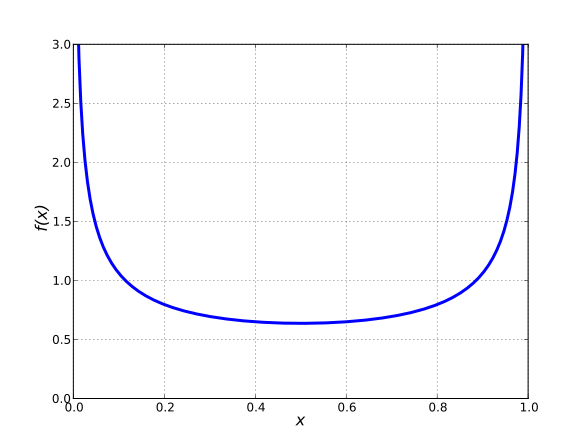
\includegraphics[width=0.6\textwidth]{images/Arcsin density.png}
        \caption{Probability density function for the arcsine distribution}
    \end{figure}




% \begin{tabularx}{\textwidth}{l | X}
    {\color{darkblue} \textbf{Params.}:} {none};\hspace{0.5cm}{\color{darkblue} \textbf{$\mathcal{W}(X)$}:} {$x \in [0,1]$};\hspace{0.5cm}{\color{darkblue} \textbf{$\mathbb{E}[X]$}:} {$\frac{1}{2}$};\hspace{0.5cm}{\color{darkblue} \textbf{$Var[X]$}:} {$\tfrac{1}{8}$};\hspace{0.5cm}\\{\color{darkblue} \textbf{$f_x$}:} {$f(x) = \frac{1}{\pi\sqrt{x(1-x)}}$}{\color{darkblue} \textbf{$F_x$}:} {$F(x) = \frac{2}{\pi}\arcsin\left(\sqrt x \right)$}
% \end{tabularx}



    
        
\subsection{Raised cosine distribution}


    \begin{figure}[H]
        \centering
        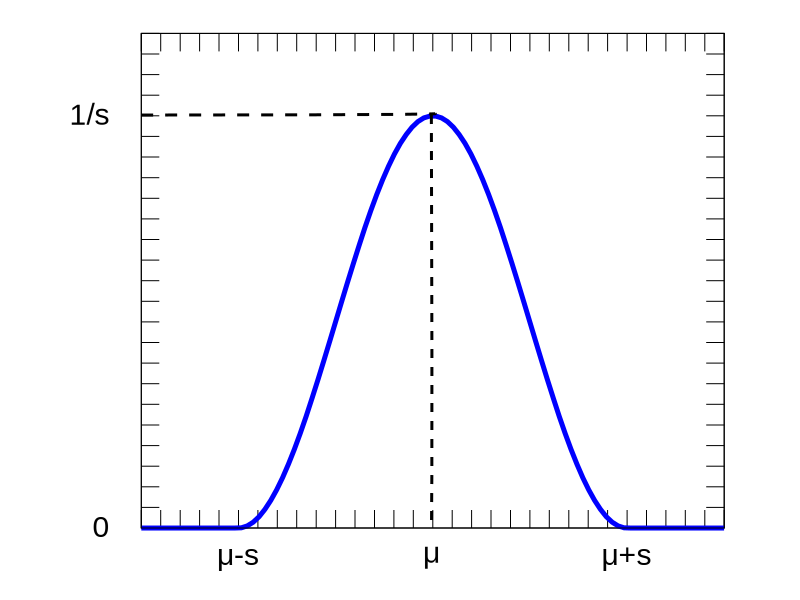
\includegraphics[width=0.6\textwidth]{images/Raised cos pdf mod.png}
        \caption{Plot of the raised cosine PDF}
    \end{figure}




% \begin{tabularx}{\textwidth}{l | X}
    {\color{darkblue} \textbf{Params.}:} {$\mu\,$ (real),  $s>0\,$ (real)};\hspace{0.5cm}{\color{darkblue} \textbf{$\mathcal{W}(X)$}:} {$x \in [\mu-s,\mu+s]\,$};\hspace{0.5cm}{\color{darkblue} \textbf{$\mathbb{E}[X]$}:} {$\mu\,$};\hspace{0.5cm}{\color{darkblue} \textbf{$Var[X]$}:} {$s^2\left(\frac{1}{3}-\frac{2}{\pi^2}\right)\,$};\hspace{0.5cm}\\{\color{darkblue} \textbf{$f_x$}:} {$$\frac{1}{2s}
\left[1+\cos\left(\frac{x-\mu}{s}\,\pi\right)\right]\,=\frac{1}{s}\operatorname{hvc}\left(\frac{x-\mu}{s}\,\pi\right)\,$$}{\color{darkblue} \textbf{$F_x$}:} {$$\frac{1}{2}\left[1+\frac{x-\mu}{s}
+\frac{1}{\pi}\sin\left(\frac{x-\mu}{s}\,\pi\right)\right]$$}
% \end{tabularx}



    
        
\subsection{Balding–Nichols model}


    \begin{figure}[H]
        \centering
        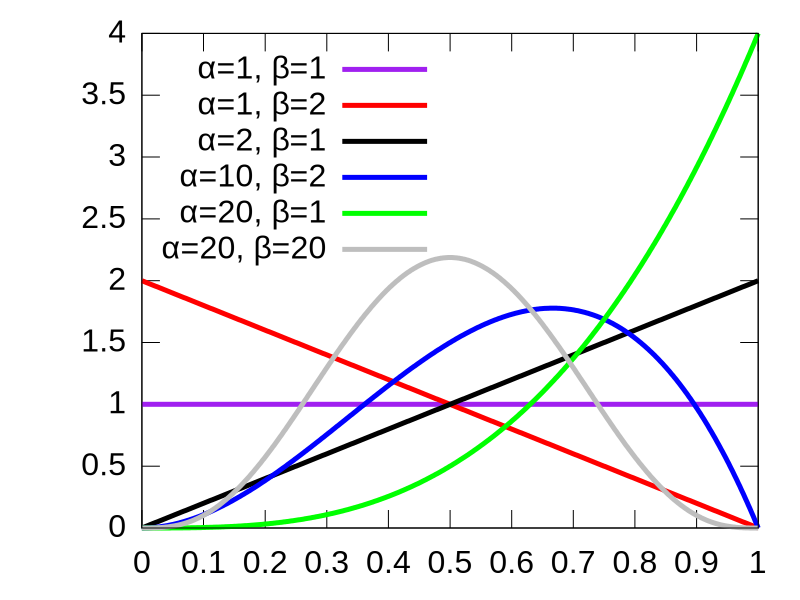
\includegraphics[width=0.6\textwidth]{images/Balding_nichols_pdf.png}
        \caption{352px}
    \end{figure}




% \begin{tabularx}{\textwidth}{l | X}
    {\color{darkblue} \textbf{Params.}:} {$0 < F < 1$ (real),  $0< p < 1$ (real),  For ease of notation, let,  $\alpha=\tfrac{1-F}{F}p$ , and ,  $\beta=\tfrac{1-F}{F}(1-p)$};\hspace{0.5cm}{\color{darkblue} \textbf{$\mathcal{W}(X)$}:} {$x \in (0; 1)\!$};\hspace{0.5cm}{\color{darkblue} \textbf{$\mathbb{E}[X]$}:} {$p\!$};\hspace{0.5cm}{\color{darkblue} \textbf{$Var[X]$}:} {$Fp(1-p)\!$};\hspace{0.5cm}\\{\color{darkblue} \textbf{$f_x$}:} {$\frac{x^{\alpha-1}(1-x)^{\beta-1}} {\mathrm{B}(\alpha,\beta)}\!$}{\color{darkblue} \textbf{$F_x$}:} {$I_x(\alpha,\beta)\!$}
% \end{tabularx}



    
        
\subsection{Uniform distribution (continuous)}


    \begin{figure}[H]
        \centering
        \includegraphics[width=0.6\textwidth]{images/Uniform Distribution PDF SVG.png}
        \caption{the maximum convention}
    \end{figure}




% \begin{tabularx}{\textwidth}{l | X}
    {\color{darkblue} \textbf{Params.}:} {$-\infty < a < b < \infty \,$};\hspace{0.5cm}{\color{darkblue} \textbf{Not.}:} {$\mathcal{U}(a, b)$ or $\mathrm{unif}(a,b)$};\hspace{0.5cm}{\color{darkblue} \textbf{$\mathcal{W}(X)$}:} {$x \in [a,b]$};\hspace{0.5cm}{\color{darkblue} \textbf{$\mathbb{E}[X]$}:} {$\tfrac{1}{2}(a+b)$};\hspace{0.5cm}{\color{darkblue} \textbf{$Var[X]$}:} {$\tfrac{1}{12}(b-a)^2$};\hspace{0.5cm}\\{\color{darkblue} \textbf{$f_x$}:} {$$\begin{cases}
                  \frac{1}{b - a} & \text{for } x \in [a,b]  \\
                  0               & \text{otherwise}
                \end{cases}$$}{\color{darkblue} \textbf{$F_x$}:} {$$\begin{cases}
                  0               & \text{for } x < a \\
                  \frac{x-a}{b-a} & \text{for } x \in [a,b] \\
                  1               & \text{for } x > b
                \end{cases}$$}
% \end{tabularx}



    
        
\subsection{Kumaraswamy distribution}


    \begin{figure}[H]
        \centering
        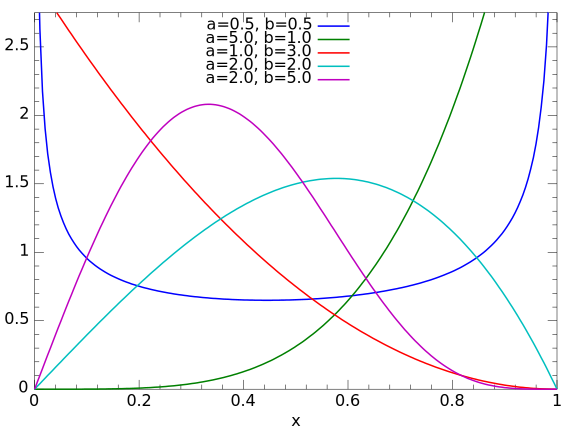
\includegraphics[width=0.6\textwidth]{images/KumaraswamyT pdf.png}
        \caption{Probability density function}
    \end{figure}




% \begin{tabularx}{\textwidth}{l | X}
    {\color{darkblue} \textbf{Params.}:} {$a>0\,$ (real),  $b>0\,$ (real)};\hspace{0.5cm}{\color{darkblue} \textbf{$\mathcal{W}(X)$}:} {$x \in (0,1)\,$};\hspace{0.5cm}{\color{darkblue} \textbf{$\mathbb{E}[X]$}:} {$\frac{b\Gamma(1+\tfrac{1}{a})\Gamma(b)}{\Gamma(1+\tfrac{1}{a}+b)}\,$};\hspace{0.5cm}{\color{darkblue} \textbf{$Var[X]$}:} {(complicated-see text)};\hspace{0.5cm}\\{\color{darkblue} \textbf{$f_x$}:} {$abx^{a-1}(1-x^a)^{b-1}\,$}{\color{darkblue} \textbf{$F_x$}:} {$1-(1-x^a)^b$}
% \end{tabularx}



    
        
\subsection{Irwin–Hall distribution}


    \begin{figure}[H]
        \centering
        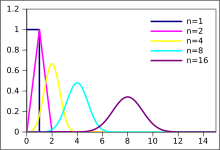
\includegraphics[width=0.6\textwidth]{images/irwin-hall-pdf.png}
        \caption{Probability mass function for the distribution}
    \end{figure}




% \begin{tabularx}{\textwidth}{l | X}
    {\color{darkblue} \textbf{Params.}:} {\textit{n} ∈ \textbf{N}\textsubscript{0}};\hspace{0.5cm}{\color{darkblue} \textbf{$\mathcal{W}(X)$}:} {$x \in [0,n]$};\hspace{0.5cm}{\color{darkblue} \textbf{$\mathbb{E}[X]$}:} {$\frac{n}{2}$};\hspace{0.5cm}{\color{darkblue} \textbf{$Var[X]$}:} {$\frac{n}{12}$};\hspace{0.5cm}\\{\color{darkblue} \textbf{$f_x$}:} {$\frac{1}{(n-1)!}\sum_{k=0}^{\lfloor x\rfloor}(-1)^k\binom{n}{k}(x-k)^{n-1}$}{\color{darkblue} \textbf{$F_x$}:} {$\frac{1}{n!}\sum_{k=0}^{\lfloor x\rfloor}(-1)^k\binom{n}{k}(x-k)^n$}
% \end{tabularx}



    
        
\subsection{Wigner semicircle distribution}


    \begin{figure}[H]
        \centering
        \includegraphics[width=0.6\textwidth]{images/WignerS distribution PDF.png}
        \caption{Plot of the Wigner semicircle PDF}
    \end{figure}




% \begin{tabularx}{\textwidth}{l | X}
    {\color{darkblue} \textbf{Params.}:} {$R>0\!$ radius (real)};\hspace{0.5cm}{\color{darkblue} \textbf{$\mathcal{W}(X)$}:} {$x \in [-R;+R]\!$};\hspace{0.5cm}{\color{darkblue} \textbf{$\mathbb{E}[X]$}:} {$0\,$};\hspace{0.5cm}{\color{darkblue} \textbf{$Var[X]$}:} {$\frac{R^2}{4}\!$};\hspace{0.5cm}\\{\color{darkblue} \textbf{$f_x$}:} {$\frac2{\pi R^2}\,\sqrt{R^2-x^2}\!$}{\color{darkblue} \textbf{$F_x$}:} {$\frac12+\frac{x\sqrt{R^2-x^2}}{\pi R^2} + \frac{\arcsin\!\left(\frac{x}{R}\right)}{\pi}\!$ , for $-R\leq x \leq R$}
% \end{tabularx}



    
        
\subsection{Reciprocal distribution}


    \begin{figure}[H]
        \centering
        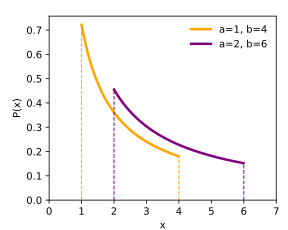
\includegraphics[width=0.6\textwidth]{images/Reciprocal pdf.png}
        \caption{Probability density function}
    \end{figure}




% \begin{tabularx}{\textwidth}{l | X}
    {\color{darkblue} \textbf{Params.}:} {$ 0 < a < b, a, b \in \R$};\hspace{0.5cm}{\color{darkblue} \textbf{$\mathcal{W}(X)$}:} {$ [ a , b ] $};\hspace{0.5cm}{\color{darkblue} \textbf{$\mathbb{E}[X]$}:} {$\frac{b-a}{\ln\frac ba}$};\hspace{0.5cm}{\color{darkblue} \textbf{$Var[X]$}:} {$\frac{b^2-a^2}{2\ln\frac ba}-\left(\frac{b-a}{\ln\frac ba}\right)^2$};\hspace{0.5cm}\\{\color{darkblue} \textbf{$f_x$}:} {$\frac1{x\ln\frac ba}$}{\color{darkblue} \textbf{$F_x$}:} {$\log_{\frac ba}\frac xa$}
% \end{tabularx}



    
        
\subsection{Beta distribution}


    \begin{figure}[H]
        \centering
        \includegraphics[width=0.6\textwidth]{images/Beta distribution pdf.png}
        \caption{Probability density function for the Beta distribution}
    \end{figure}




% \begin{tabularx}{\textwidth}{l | X}
    {\color{darkblue} \textbf{Params.}:} {\textit{α} > 0 shape (real), \textit{β} > 0 shape (real)};\hspace{0.5cm}{\color{darkblue} \textbf{Not.}:} {Beta(\textit{α}, \textit{β})};\hspace{0.5cm}{\color{darkblue} \textbf{$\mathcal{W}(X)$}:} {$x \in [0, 1]\!$ or $x \in (0, 1)\!$};\hspace{0.5cm}{\color{darkblue} \textbf{$\mathbb{E}[X]$}:} {$\operatorname{E}[X] = \frac{\alpha}{\alpha+\beta}\!$ ,  $\operatorname{E}[\ln X] = \psi(\alpha) - \psi(\alpha + \beta)\!$ , ,  $\operatorname{E}[X \, \ln X] = \frac{\alpha}{\alpha+\beta}\,\left[\psi(\alpha+1)-\psi(\alpha+\beta+1)\right]\!$ , (see digamma function and see section: Geometric mean)};\hspace{0.5cm}{\color{darkblue} \textbf{$Var[X]$}:} {$\operatorname{var}[X] = \frac{\alpha\beta}{(\alpha+\beta)^2(\alpha+\beta+1)}\!$ ,  $\operatorname{var}[\ln X] = \psi_1(\alpha) - \psi_1(\alpha + \beta)\!$ , (see trigamma function and see section: Geometric variance)};\hspace{0.5cm}\\{\color{darkblue} \textbf{$f_x$}:} {$\frac{x^{\alpha-1}(1-x)^{\beta-1}} {\Beta(\alpha,\beta)}\!$ , where $\Beta(\alpha,\beta) = \frac{\Gamma(\alpha)\Gamma(\beta)}{\Gamma(\alpha + \beta)}$ and $\Gamma$ is the Gamma function.}{\color{darkblue} \textbf{$F_x$}:} {$I_x(\alpha,\beta)\!$ (the regularized incomplete beta function)}
% \end{tabularx}



    
        
\subsection{Logit-normal distribution}


    \begin{figure}[H]
        \centering
        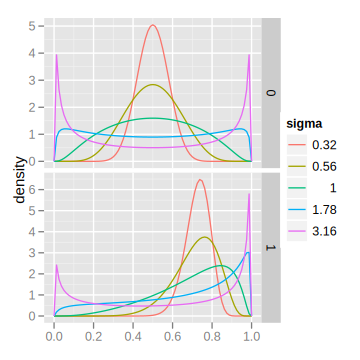
\includegraphics[width=0.6\textwidth]{images/LogitnormalPDF.png}
        \caption{Plot of the Logitnormal PDF}
    \end{figure}




% \begin{tabularx}{\textwidth}{l | X}
    {\color{darkblue} \textbf{Params.}:} {\textit{σ}\textsuperscript{2} > 0 — squared scale (real),,  \textit{μ} ∈ \textbf{R} — location};\hspace{0.5cm}{\color{darkblue} \textbf{Not.}:} {$P( \mathcal{N}(\mu,\,\sigma^2) )$};\hspace{0.5cm}{\color{darkblue} \textbf{$\mathcal{W}(X)$}:} {\textit{x} ∈ (0, 1)};\hspace{0.5cm}{\color{darkblue} \textbf{$\mathbb{E}[X]$}:} {no analytical solution};\hspace{0.5cm}{\color{darkblue} \textbf{$Var[X]$}:} {no analytical solution};\hspace{0.5cm}\\{\color{darkblue} \textbf{$f_x$}:} {$\frac{1}{\sigma \sqrt{2 \pi}}\, e^{-\frac{(\operatorname{logit}(x) - \mu)^2}{2\sigma^2}}\frac{1}{x (1-x)}$}{\color{darkblue} \textbf{$F_x$}:} {$\frac12\Big[1 + \operatorname{erf}\Big( \frac{\operatorname{logit}(x)-\mu}{\sqrt{2\sigma^2}}\Big)\Big]$}
% \end{tabularx}



    
        
\subsection{Bates distribution}


    \begin{figure}[H]
        \centering
        \includegraphics[width=0.6\textwidth]{images/batesPDF.png}
        \caption{325px}
    \end{figure}




% \begin{tabularx}{\textwidth}{l | X}
    {\color{darkblue} \textbf{Params.}:} {$-\infty < a < b < \infty $ ,  $ n \geq 1 $ integer};\hspace{0.5cm}{\color{darkblue} \textbf{$\mathcal{W}(X)$}:} {$x \in [a,b]$};\hspace{0.5cm}{\color{darkblue} \textbf{$\mathbb{E}[X]$}:} {$\tfrac{1}{2}(a+b)$};\hspace{0.5cm}{\color{darkblue} \textbf{$Var[X]$}:} {$\tfrac{1}{12n}(b-a)^2$};\hspace{0.5cm}\\{\color{darkblue} \textbf{$f_x$}:} {see below}
% \end{tabularx}



    
        
\subsection{ARGUS distribution}


    \begin{figure}[H]
        \centering
        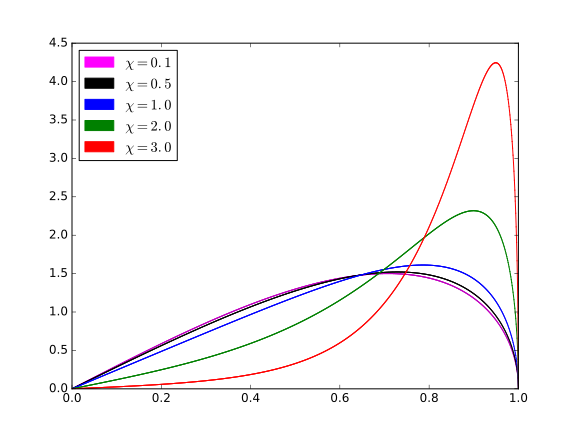
\includegraphics[width=0.6\textwidth]{images/argusPDF.png}
        \caption{325px}
    \end{figure}




% \begin{tabularx}{\textwidth}{l | X}
    {\color{darkblue} \textbf{Params.}:} {$c > 0$ cut-off (real),  $\chi > 0$ curvature (real)};\hspace{0.5cm}{\color{darkblue} \textbf{$\mathcal{W}(X)$}:} {$x \in (0, c)\!$};\hspace{0.5cm}{\color{darkblue} \textbf{$\mathbb{E}[X]$}:} {$\mu = c\sqrt{\pi/8}\;\frac{\chi e^{-\frac{\chi^2}{4}} I_1(\tfrac{\chi^2}{4})}{ \Psi(\chi) }$ , ,  where \textit{I}\textsubscript{1} is the Modified Bessel function of the first kind of order 1, and $\Psi(x)$ is given in the text.};\hspace{0.5cm}{\color{darkblue} \textbf{$Var[X]$}:} {$c^2\!\left(1 - \frac{3}{\chi^2} + \frac{\chi\phi(\chi)}{\Psi(\chi)}\right) - \mu^2$};\hspace{0.5cm}\\{\color{darkblue} \textbf{$f_x$}:} {see text}{\color{darkblue} \textbf{$F_x$}:} {see text}
% \end{tabularx}



    


    \section{Continuous univariate supported on a semi-infinite interval}
        

        
    
        
\subsection{Discrete Weibull distribution}





% \begin{tabularx}{\textwidth}{l | X}
    {\color{darkblue} \textbf{Params.}:} {$\alpha> 0 $ scale ,  $\beta >0 $ shape};\hspace{0.5cm}{\color{darkblue} \textbf{$\mathcal{W}(X)$}:} {$x \in \{0, 1,2,\ldots\}$};\hspace{0.5cm}\\{\color{darkblue} \textbf{$f_x$}:} {$$\exp\left[-\left(\frac{x  }{\alpha}\right)^\beta \right]-
  	\exp\left[-\left(\frac{x+1}{\alpha}\right)^\beta \right]$$}{\color{darkblue} \textbf{$F_x$}:} {$1-\exp\left[-\left(\frac{x+1}{\alpha}\right)^\beta \right]$}
% \end{tabularx}



    
        
\subsection{Benktander type I distribution}





% \begin{tabularx}{\textwidth}{l | X}
    {\color{darkblue} \textbf{Params.}:} {$a>0$ (real),  $b>0$ real};\hspace{0.5cm}{\color{darkblue} \textbf{$\mathcal{W}(X)$}:} {$x\geq 1$};\hspace{0.5cm}{\color{darkblue} \textbf{$\mathbb{E}[X]$}:} {$1+\tfrac{1}{a}$};\hspace{0.5cm}{\color{darkblue} \textbf{$Var[X]$}:} {$ \frac{-\sqrt{b}+ae^{\frac{(a-1)^2}{4b}}\sqrt{\pi}\;\textrm{erfc}\left(\frac{a-1}{2\sqrt{b}}\right)}{a^2\sqrt{b}}$};\hspace{0.5cm}\\{\color{darkblue} \textbf{$f_x$}:} {$ \left(\left[\left(1+\frac{2b\log x}{a}\right)\left(1+a+2b\log x\right)\right]-\frac{2b}{a}\right)x^{-\left(2+a+b\log x\right)} $}{\color{darkblue} \textbf{$F_x$}:} {$ 1 - \left(1+\frac{2b}{a}\log x\right)x^{-\left(a + 1 + b\log x\right)} $}
% \end{tabularx}



    
        
\subsection{Davis distribution}





% \begin{tabularx}{\textwidth}{l | X}
    {\color{darkblue} \textbf{Params.}:} {$b>0$ scale,  $ n> 0$ shape,  $\mu>0$ location};\hspace{0.5cm}{\color{darkblue} \textbf{$\mathcal{W}(X)$}:} {$x>\mu$};\hspace{0.5cm}{\color{darkblue} \textbf{$\mathbb{E}[X]$}:} {$$\begin{cases}
              \mu + \frac{b\zeta(n-1)}{(n-1)\zeta(n)} & \text{if}\ n>2    \\
              \text{Indeterminate} & \text{otherwise}\ \end{cases}$$};\hspace{0.5cm}{\color{darkblue} \textbf{$Var[X]$}:} {$$\begin{cases}
              \frac{ b^2 \left( -(n-2){\zeta(n-1)}^2+(n-1)\zeta(n-2)\zeta(n) \right)}{(n-2) {(n-1)}^2 {\zeta(n)}^2} & \text{if}\ n>3    \\
              \text{Indeterminate} & \text{otherwise}\ \end{cases}$$};\hspace{0.5cm}\\{\color{darkblue} \textbf{$f_x$}:} {$ \frac{ b^n {(x-\mu)}^{-1-n} }{ \left( e^{\frac{b}{x-\mu}} -1 \right) \Gamma(n) \zeta(n) } $ ,  Where $\Gamma(n)$ is the Gamma function and $\zeta(n)$ is the Riemann zeta function}
% \end{tabularx}



    
        
\subsection{Benini distribution}





% \begin{tabularx}{\textwidth}{l | X}
    {\color{darkblue} \textbf{Params.}:} {$\alpha>0$ shape (real),  $\beta>0$ shape (real),  $\sigma>0$ scale (real)};\hspace{0.5cm}{\color{darkblue} \textbf{$\mathcal{W}(X)$}:} {$x>\sigma$};\hspace{0.5cm}{\color{darkblue} \textbf{$\mathbb{E}[X]$}:} {$\sigma+\tfrac{\sigma}{\sqrt{2\beta}} H_{-1}\left(\tfrac{-1+\alpha}{\sqrt{2\beta}}\right) $ ,  where $H_n(x)$ is the \textbf{"probabilists' Hermite polynomials"}};\hspace{0.5cm}{\color{darkblue} \textbf{$Var[X]$}:} {$\left(\sigma^2+\tfrac{2\sigma^2}{\sqrt{2\beta}} H_{-1}\left(\tfrac{-2+\alpha}{\sqrt{2\beta}}\right)\right)-\mu^2 $};\hspace{0.5cm}\\{\color{darkblue} \textbf{$f_x$}:} {$e^{-\alpha\log{\frac{x}{\sigma}}-\beta\left[\log{\frac{x}{\sigma}}\right]^2} \left(\frac{\alpha}{x}+\frac{2\beta\log{\frac{x}{\sigma}}}{x}\right) $}{\color{darkblue} \textbf{$F_x$}:} {$1-e^{-\alpha\log{\frac{x}{\sigma}}-\beta[\log{\frac{x}{\sigma}}]^2}$}
% \end{tabularx}



    
        
\subsection{Type-2 Gumbel distribution}





% \begin{tabularx}{\textwidth}{l | X}
    {\color{darkblue} \textbf{Params.}:} {$a\!$ (real),  $b\!$ shape (real)};\hspace{0.5cm}{\color{darkblue} \textbf{$\mathbb{E}[X]$}:} {$ b^{1/a}\Gamma(1-1/a)\!$};\hspace{0.5cm}{\color{darkblue} \textbf{$Var[X]$}:} {$b^{2/a}(\Gamma(1-1/a)-{\Gamma(1-1/a)}^2)\!$};\hspace{0.5cm}\\{\color{darkblue} \textbf{$f_x$}:} {$ a b x^{-a-1} e^{-b x^{-a}}\!$}{\color{darkblue} \textbf{$F_x$}:} {$ e^{-b x^{-a}}\!$}
% \end{tabularx}



    
        
\subsection{Hypoexponential distribution}





% \begin{tabularx}{\textwidth}{l | X}
    {\color{darkblue} \textbf{Params.}:} {$\lambda_{1},\dots,\lambda_{k} > 0\,$ rates (real)};\hspace{0.5cm}{\color{darkblue} \textbf{$\mathcal{W}(X)$}:} {$x \in [0; \infty)\!$};\hspace{0.5cm}{\color{darkblue} \textbf{$\mathbb{E}[X]$}:} {$\sum^{k}_{i=1}1/\lambda_{i}\,$};\hspace{0.5cm}{\color{darkblue} \textbf{$Var[X]$}:} {$\sum^{k}_{i=1}1/\lambda^2_{i}$};\hspace{0.5cm}\\{\color{darkblue} \textbf{$f_x$}:} {Expressed as a phase-type distribution,  $-\boldsymbol{\alpha}e^{x\Theta}\Theta\boldsymbol{1}$ , Has no other simple form; see article for details}{\color{darkblue} \textbf{$F_x$}:} {Expressed as a phase-type distribution,  $1-\boldsymbol{\alpha}e^{x\Theta}\boldsymbol{1}$}
% \end{tabularx}



    
        
\subsection{Phase-type distribution}





% \begin{tabularx}{\textwidth}{l | X}
    {\color{darkblue} \textbf{Params.}:} {$S,\; m\times m$ subgenerator matrix,  $\boldsymbol{\alpha}$ , probability row vector};\hspace{0.5cm}{\color{darkblue} \textbf{$\mathcal{W}(X)$}:} {$x \in [0; \infty)\!$};\hspace{0.5cm}{\color{darkblue} \textbf{$\mathbb{E}[X]$}:} {$-\boldsymbol{\alpha}{S}^{-1}\mathbf{1}$};\hspace{0.5cm}{\color{darkblue} \textbf{$Var[X]$}:} {$2\boldsymbol{\alpha}{S}^{-2}\mathbf{1}-(\boldsymbol{\alpha}{S}^{-1}\mathbf{1})^{2}$};\hspace{0.5cm}\\{\color{darkblue} \textbf{$f_x$}:} {$\boldsymbol{\alpha}e^{xS}\boldsymbol{S}^{0}$ ,  See article for details}{\color{darkblue} \textbf{$F_x$}:} {$1-\boldsymbol{\alpha}e^{xS}\boldsymbol{1}$}
% \end{tabularx}



    
        
\subsection{Log-logistic distribution}





% \begin{tabularx}{\textwidth}{l | X}
    {\color{darkblue} \textbf{Params.}:} {$\alpha>0$ scale,  $\beta> 0$ shape};\hspace{0.5cm}{\color{darkblue} \textbf{$\mathcal{W}(X)$}:} {$x\in[0,\infty)$};\hspace{0.5cm}{\color{darkblue} \textbf{$\mathbb{E}[X]$}:} {${\alpha\,\pi/\beta \over \sin(\pi/\beta)}$ , if $\beta>1$ , else undefined};\hspace{0.5cm}{\color{darkblue} \textbf{$Var[X]$}:} {See main text};\hspace{0.5cm}\\{\color{darkblue} \textbf{$f_x$}:} {$$\frac{ (\beta/\alpha)(x/\alpha)^{\beta-1} }
                       { \left (1+(x/\alpha)^{\beta} \right)^2  }$$}{\color{darkblue} \textbf{$F_x$}:} {${ 1 \over 1+(x/\alpha)^{-\beta} }$}
% \end{tabularx}



    
        
\subsection{Log-Cauchy distribution}





% \begin{tabularx}{\textwidth}{l | X}
    {\color{darkblue} \textbf{Params.}:} {$\mu$ (real),  $\displaystyle \sigma > 0\!$ (real)};\hspace{0.5cm}{\color{darkblue} \textbf{$\mathcal{W}(X)$}:} {$\displaystyle x \in (0, +\infty)\!$};\hspace{0.5cm}{\color{darkblue} \textbf{$\mathbb{E}[X]$}:} {infinite};\hspace{0.5cm}{\color{darkblue} \textbf{$Var[X]$}:} {infinite};\hspace{0.5cm}\\{\color{darkblue} \textbf{$f_x$}:} {${ 1 \over x\pi } \left[ { \sigma \over (\ln x - \mu)^2 + \sigma^2  } \right], \ \ x>0$}{\color{darkblue} \textbf{$F_x$}:} {$\frac{1}{\pi} \arctan\left(\frac{\ln x-\mu}{\sigma}\right)+\frac{1}{2}, \ \ x>0$}
% \end{tabularx}



    
        
\subsection{Noncentral chi-squared distribution}


    \begin{figure}[H]
        \centering
        \includegraphics[width=0.6\textwidth]{images/Chi-Squared-(nonCentral)-pdf.png}
        \caption{325px}
    \end{figure}




% \begin{tabularx}{\textwidth}{l | X}
    {\color{darkblue} \textbf{Params.}:} {$k > 0\,$ degrees of freedom,  $\lambda > 0\,$ non-centrality parameter};\hspace{0.5cm}{\color{darkblue} \textbf{$\mathcal{W}(X)$}:} {$x \in [0; +\infty)\,$};\hspace{0.5cm}{\color{darkblue} \textbf{$\mathbb{E}[X]$}:} {$k+\lambda\,$};\hspace{0.5cm}{\color{darkblue} \textbf{$Var[X]$}:} {$2(k+2\lambda)\,$};\hspace{0.5cm}\\{\color{darkblue} \textbf{$f_x$}:} {$$\frac{1}{2}e^{-(x+\lambda)/2}\left (\frac{x}{\lambda} \right)^{k/4-1/2}
 I_{k/2-1}(\sqrt{\lambda x})$$}{\color{darkblue} \textbf{$F_x$}:} {$1 - Q_{\frac{k}{2}} \left( \sqrt{\lambda}, \sqrt{x} \right)$ with Marcum Q-function $Q_M(a,b)$}
% \end{tabularx}



    
        
\subsection{Dagum distribution}


    \begin{figure}[H]
        \centering
        \includegraphics[width=0.6\textwidth]{images/DagumPDF.png}
        \caption{The pdf of the Dagum distribution for various parameter specifications.}
    \end{figure}




% \begin{tabularx}{\textwidth}{l | X}
    {\color{darkblue} \textbf{Params.}:} {$p>0$ shape  ,  $a>0$ shape ,  $b > 0$ scale};\hspace{0.5cm}{\color{darkblue} \textbf{$\mathcal{W}(X)$}:} {$x>0$};\hspace{0.5cm}{\color{darkblue} \textbf{$\mathbb{E}[X]$}:} {$$\begin{cases}
              -\frac{b}{a}\frac{\Gamma\left(-\tfrac{1}{a}\right)\Gamma\left(\tfrac{1}{a}+p\right)}{\Gamma(p)} & \text{if}\ a>1    \\
              \text{Indeterminate} & \text{otherwise}\ \end{cases}$$};\hspace{0.5cm}{\color{darkblue} \textbf{$Var[X]$}:} {$$\begin{cases}
              -\frac{b^2}{a^2} \left(2 a \frac{\Gamma\left(-\tfrac{2}{a}\right) \, \Gamma\left(\tfrac{2}{a} + p\right)}{\Gamma\left(p\right)} + \left( \frac{\Gamma\left(-\tfrac{1}{a}\right) \Gamma\left(\tfrac{1}{a} + p\right)}{\Gamma\left(p\right)} \right)^2\right) & \text{if}\ a>2    \\
              \text{Indeterminate} & \text{otherwise}\ \end{cases}$$};\hspace{0.5cm}\\{\color{darkblue} \textbf{$f_x$}:} {$ \frac{a p}{x} \left( \frac{(\tfrac{x}{b})^{a p}}{\left((\tfrac{x}{b})^a + 1 \right)^{p+1}} \right) $}{\color{darkblue} \textbf{$F_x$}:} {$ {\left( 1+{\left(\frac{x}{b}\right)}^{-a} \right)}^{-p} $}
% \end{tabularx}



    
        
\subsection{Inverse-chi-squared distribution}


    \begin{figure}[H]
        \centering
        \includegraphics[width=0.6\textwidth]{images/Inverse chi squared density.png}
        \caption{}
    \end{figure}




% \begin{tabularx}{\textwidth}{l | X}
    {\color{darkblue} \textbf{Params.}:} {$\nu > 0\!$};\hspace{0.5cm}{\color{darkblue} \textbf{$\mathcal{W}(X)$}:} {$x \in (0, \infty)\!$};\hspace{0.5cm}{\color{darkblue} \textbf{$\mathbb{E}[X]$}:} {$\frac{1}{\nu-2}\!$ for $\nu >2\!$};\hspace{0.5cm}{\color{darkblue} \textbf{$Var[X]$}:} {$\frac{2}{(\nu-2)^2 (\nu-4)}\!$ for $\nu >4\!$};\hspace{0.5cm}\\{\color{darkblue} \textbf{$f_x$}:} {$\frac{2^{-\nu/2}}{\Gamma(\nu/2)}\,x^{-\nu/2-1}  e^{-1/(2 x)}\!$}{\color{darkblue} \textbf{$F_x$}:} {$$\Gamma\!\left(\frac{\nu}{2},\frac{1}{2x}\right)
\bigg/\, \Gamma\!\left(\frac{\nu}{2}\right)\!$$}
% \end{tabularx}



    
        
\subsection{Generalized gamma distribution}


    \begin{figure}[H]
        \centering
        \includegraphics[width=0.6\textwidth]{images/GenGamma.png}
        \caption{Gen Gamma PDF plot}
    \end{figure}




% \begin{tabularx}{\textwidth}{l | X}
    {\color{darkblue} \textbf{Params.}:} {$a>0$ (scale), $d>0, p>0$};\hspace{0.5cm}{\color{darkblue} \textbf{$\mathcal{W}(X)$}:} {$x \;\in\; (0,\, \infty)$};\hspace{0.5cm}{\color{darkblue} \textbf{$\mathbb{E}[X]$}:} {$a \frac{\Gamma((d+1)/p)}{\Gamma(d/p)}$};\hspace{0.5cm}{\color{darkblue} \textbf{$Var[X]$}:} {$a^2\left(\frac{\Gamma((d+2)/p)}{\Gamma(d/p)} - \left(\frac{\Gamma((d+1)/p)}{\Gamma(d/p)}\right)^2\right)$};\hspace{0.5cm}\\{\color{darkblue} \textbf{$f_x$}:} {$\frac{p/a^d}{\Gamma(d/p)} x^{d-1}e^{-(x/a)^p}$}{\color{darkblue} \textbf{$F_x$}:} {$\frac{\gamma(d/p, (x/a)^p)}{\Gamma(d/p)}$}
% \end{tabularx}



    
        
\subsection{Rice distribution}


    \begin{figure}[H]
        \centering
        \includegraphics[width=0.6\textwidth]{images/Rice distributiona PDF.png}
        \caption{Rice probability density functions σ = 1.0}
    \end{figure}




% \begin{tabularx}{\textwidth}{l | X}
    {\color{darkblue} \textbf{Params.}:} {$\nu\ge 0$ , distance between the reference point and the center of the bivariate distribution,,  $\sigma\ge 0$ , spread};\hspace{0.5cm}{\color{darkblue} \textbf{$\mathcal{W}(X)$}:} {$x \in [0,\infty)$};\hspace{0.5cm}{\color{darkblue} \textbf{$\mathbb{E}[X]$}:} {$\sigma  \sqrt{\pi/2}\,\,L_{1/2}(-\nu^2/2\sigma^2)$};\hspace{0.5cm}{\color{darkblue} \textbf{$Var[X]$}:} {$2\sigma^2+\nu^2-\frac{\pi\sigma^2}{2}L_{1/2}^2\left(\frac{-\nu^2}{2\sigma^2}\right)$};\hspace{0.5cm}\\{\color{darkblue} \textbf{$f_x$}:} {$$\frac{x}{\sigma^2}\exp\left(\frac{-(x^2+\nu^2)}
{2\sigma^2}\right)I_0\left(\frac{x\nu}{\sigma^2}\right)$$}{\color{darkblue} \textbf{$F_x$}:} {$1-Q_1\left(\frac{\nu}{\sigma },\frac{x}{\sigma }\right)$ where \textit{Q}\textsubscript{1} is the Marcum Q-function}
% \end{tabularx}



    
        
\subsection{Scaled inverse chi-squared distribution}


    \begin{figure}[H]
        \centering
        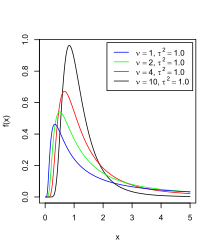
\includegraphics[width=0.6\textwidth]{images/Scaled inverse chi squared.png}
        \caption{250px}
    \end{figure}




% \begin{tabularx}{\textwidth}{l | X}
    {\color{darkblue} \textbf{Params.}:} {$\nu > 0\,$ ,  $\tau^2 > 0\,$};\hspace{0.5cm}{\color{darkblue} \textbf{$\mathcal{W}(X)$}:} {$x \in (0, \infty)$};\hspace{0.5cm}{\color{darkblue} \textbf{$\mathbb{E}[X]$}:} {$\frac{\nu \tau^2}{\nu-2}$ for $\nu >2\,$};\hspace{0.5cm}{\color{darkblue} \textbf{$Var[X]$}:} {$\frac{2 \nu^2 \tau^4}{(\nu-2)^2 (\nu-4)}$ for $\nu >4\,$};\hspace{0.5cm}\\{\color{darkblue} \textbf{$f_x$}:} {$$\frac{(\tau^2\nu/2)^{\nu/2}}{\Gamma(\nu/2)}~
\frac{\exp\left[ \frac{-\nu \tau^2}{2 x}\right]}{x^{1+\nu/2}}$$}{\color{darkblue} \textbf{$F_x$}:} {$$\Gamma\left(\frac{\nu}{2},\frac{\tau^2\nu}{2x}\right)
\left/\Gamma\left(\frac{\nu}{2}\right)\right.$$}
% \end{tabularx}



    
        
\subsection{Beta prime distribution}


    \begin{figure}[H]
        \centering
        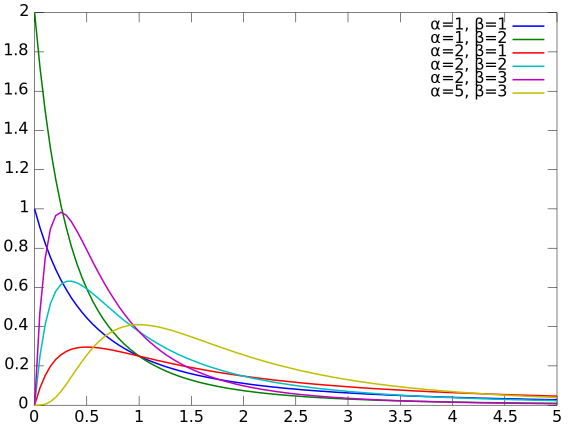
\includegraphics[width=0.6\textwidth]{images/Beta prime pdf.png}
        \caption{325px}
    \end{figure}




% \begin{tabularx}{\textwidth}{l | X}
    {\color{darkblue} \textbf{Params.}:} {$\alpha > 0$ shape (real),  $\beta > 0$ shape (real)};\hspace{0.5cm}{\color{darkblue} \textbf{$\mathcal{W}(X)$}:} {$x \in [0,\infty)\!$};\hspace{0.5cm}{\color{darkblue} \textbf{$\mathbb{E}[X]$}:} {$\frac{\alpha}{\beta-1} \text{ if } \beta>1$};\hspace{0.5cm}{\color{darkblue} \textbf{$Var[X]$}:} {$\frac{\alpha(\alpha+\beta-1)}{(\beta-2)(\beta-1)^2} \text{ if } \beta>2$};\hspace{0.5cm}\\{\color{darkblue} \textbf{$f_x$}:} {$f(x) = \frac{x^{\alpha-1} (1+x)^{-\alpha -\beta}}{B(\alpha,\beta)}\!$}{\color{darkblue} \textbf{$F_x$}:} {$ I_{\frac{x}{1+x}(\alpha,\beta) }$ where $I_x(\alpha,\beta)$ is the incomplete beta function}
% \end{tabularx}



    
        
\subsection{Benktander type II distribution}


    \begin{figure}[H]
        \centering
        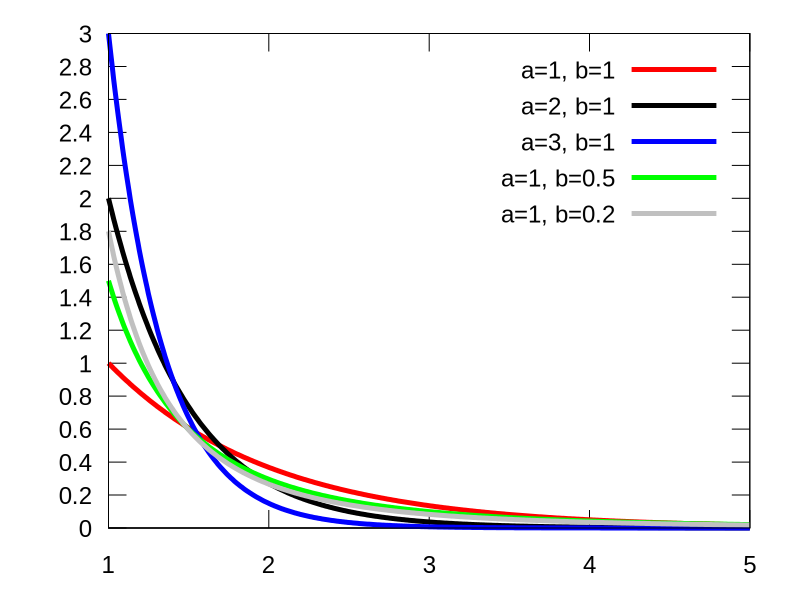
\includegraphics[width=0.6\textwidth]{images/Benktander2PDF.png}
        \caption{325px}
    \end{figure}




% \begin{tabularx}{\textwidth}{l | X}
    {\color{darkblue} \textbf{Params.}:} {$a>0$ (real),  $0<b\leq1$ (real)};\hspace{0.5cm}{\color{darkblue} \textbf{$\mathcal{W}(X)$}:} {$x \geq 1$};\hspace{0.5cm}{\color{darkblue} \textbf{$\mathbb{E}[X]$}:} {$1+\frac{1}{a}$};\hspace{0.5cm}{\color{darkblue} \textbf{$Var[X]$}:} {$ \frac{-b + 2ae^{\frac{a}{b}}\mathbf{E}_{1-\frac{1}{b}}\left(\frac{a}{b}\right)}{a^2 b}$ , Where $\mathbf{E}_n(x)$ is the generalized Exponential integral};\hspace{0.5cm}\\{\color{darkblue} \textbf{$f_x$}:} {$ e^{\frac{a}{b}(1 - x^b)}x^{b-2}\left(ax^b - b + 1\right) $}{\color{darkblue} \textbf{$F_x$}:} {$ 1 - x^{b-1}e^{\frac{a}{b}(1 - x^b)} $}
% \end{tabularx}



    
        
\subsection{Inverse-gamma distribution}


    \begin{figure}[H]
        \centering
        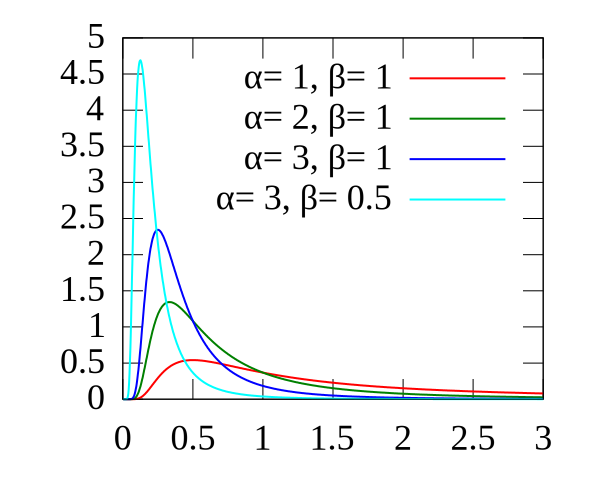
\includegraphics[width=0.6\textwidth]{images/Inv gamma pdf.png}
        \caption{325px}
    \end{figure}




% \begin{tabularx}{\textwidth}{l | X}
    {\color{darkblue} \textbf{Params.}:} {$\alpha>0$ shape (real),  $\beta>0$ scale (real)};\hspace{0.5cm}{\color{darkblue} \textbf{$\mathcal{W}(X)$}:} {$x\in(0,\infty)\!$};\hspace{0.5cm}{\color{darkblue} \textbf{$\mathbb{E}[X]$}:} {$\frac{\beta}{\alpha-1}\!$ for $\alpha > 1$};\hspace{0.5cm}{\color{darkblue} \textbf{$Var[X]$}:} {$\frac{\beta^2}{(\alpha-1)^2(\alpha-2)}\!$ for $\alpha > 2$};\hspace{0.5cm}\\{\color{darkblue} \textbf{$f_x$}:} {$\frac{\beta^\alpha}{\Gamma(\alpha)} x^{-\alpha - 1} \exp \left(-\frac{\beta}{x}\right)$}{\color{darkblue} \textbf{$F_x$}:} {$\frac{\Gamma(\alpha,\beta/x)}{\Gamma(\alpha)} \!$}
% \end{tabularx}



    
        
\subsection{Burr distribution}


    \begin{figure}[H]
        \centering
        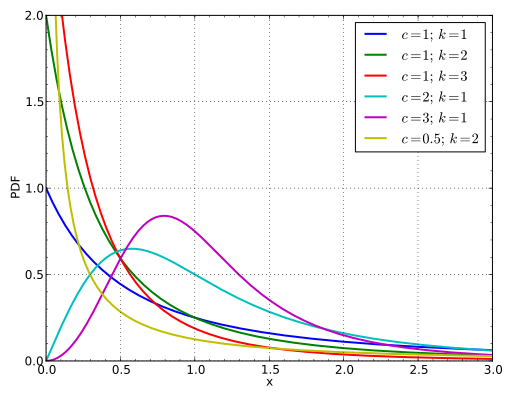
\includegraphics[width=0.6\textwidth]{images/Burr pdf.png}
        \caption{325px}
    \end{figure}




% \begin{tabularx}{\textwidth}{l | X}
    {\color{darkblue} \textbf{Params.}:} {$c > 0\!$ ,  $k > 0\!$};\hspace{0.5cm}{\color{darkblue} \textbf{$\mathcal{W}(X)$}:} {$x > 0\!$};\hspace{0.5cm}{\color{darkblue} \textbf{$\mathbb{E}[X]$}:} {$\mu_1=k\operatorname{\Beta}(k-1/c,\, 1+1/c)$ where Β() is the beta function};\hspace{0.5cm}{\color{darkblue} \textbf{$Var[X]$}:} {$-\mu_1^2+\mu_2$};\hspace{0.5cm}\\{\color{darkblue} \textbf{$f_x$}:} {$ck\frac{x^{c-1}}{(1+x^c)^{k+1}}\!$}{\color{darkblue} \textbf{$F_x$}:} {$1-\left(1+x^c\right)^{-k}$}
% \end{tabularx}



    
        
\subsection{Chi distribution}


    \begin{figure}[H]
        \centering
        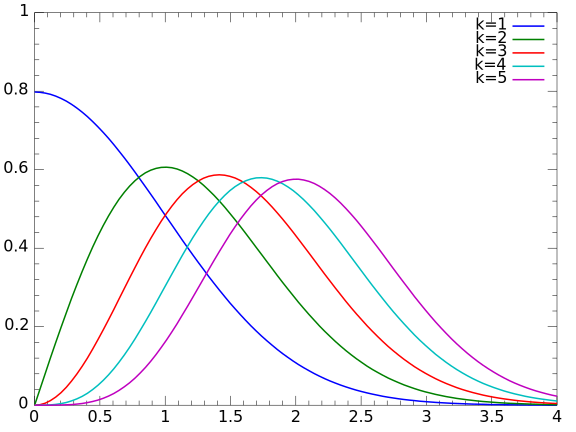
\includegraphics[width=0.6\textwidth]{images/Chi distribution PDF.png}
        \caption{Plot of the Chi PMF}
    \end{figure}




% \begin{tabularx}{\textwidth}{l | X}
    {\color{darkblue} \textbf{Params.}:} {$k>0\,$ (degrees of freedom)};\hspace{0.5cm}{\color{darkblue} \textbf{$\mathcal{W}(X)$}:} {$x\in [0,\infty)$};\hspace{0.5cm}{\color{darkblue} \textbf{$\mathbb{E}[X]$}:} {$\mu=\sqrt{2}\,\frac{\Gamma((k+1)/2)}{\Gamma(k/2)}$};\hspace{0.5cm}{\color{darkblue} \textbf{$Var[X]$}:} {$\sigma^2=k-\mu^2\,$};\hspace{0.5cm}\\{\color{darkblue} \textbf{$f_x$}:} {$\frac{1}{2^{(k/2)-1}\Gamma(k/2)}\;x^{k-1}e^{-x^2/2}$}{\color{darkblue} \textbf{$F_x$}:} {$P(k/2,x^2/2)\,$}
% \end{tabularx}



    
        
\subsection{Generalized inverse Gaussian distribution}


    \begin{figure}[H]
        \centering
        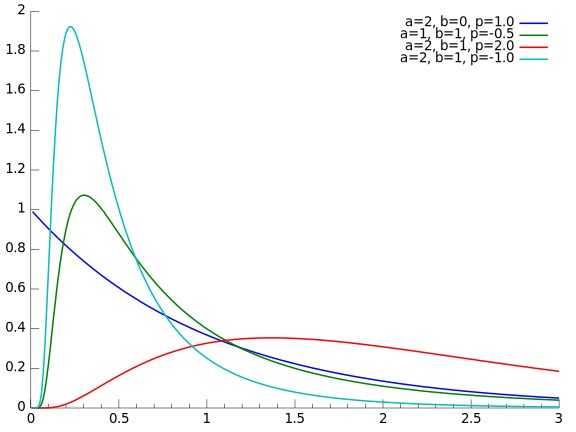
\includegraphics[width=0.6\textwidth]{images/GIG distribution pdf.png}
        \caption{Probability density plots of GIG distributions}
    \end{figure}




% \begin{tabularx}{\textwidth}{l | X}
    {\color{darkblue} \textbf{Params.}:} {\textit{a} > 0, \textit{b} > 0, \textit{p} real};\hspace{0.5cm}{\color{darkblue} \textbf{$\mathcal{W}(X)$}:} {\textit{x} > 0};\hspace{0.5cm}{\color{darkblue} \textbf{$\mathbb{E}[X]$}:} {$\operatorname{E}[x]=\frac{\sqrt{b}\ K_{p+1}(\sqrt{a b}) }{ \sqrt{a}\ K_{p}(\sqrt{a b})}$ ,  $\operatorname{E}[x^{-1}]=\frac{\sqrt{a}\ K_{p+1}(\sqrt{a b}) }{ \sqrt{b}\ K_{p}(\sqrt{a b})}-\frac{2p}{b}$ ,  $\operatorname{E}[\ln x]=\ln \frac{\sqrt{b}}{\sqrt{a}}+\frac{\partial}{\partial p} \ln K_{p}(\sqrt{a b})$};\hspace{0.5cm}{\color{darkblue} \textbf{$Var[X]$}:} {$\left(\frac{b}{a}\right)\left[\frac{K_{p+2}(\sqrt{ab})}{K_p(\sqrt{ab})}-\left(\frac{K_{p+1}(\sqrt{ab})}{K_p(\sqrt{ab})}\right)^2\right]$};\hspace{0.5cm}\\{\color{darkblue} \textbf{$f_x$}:} {$f(x) = \frac{(a/b)^{p/2}}{2 K_p(\sqrt{ab})} x^{(p-1)} e^{-(ax + b/x)/2}$}
% \end{tabularx}



    
        
\subsection{Log-normal distribution}


    \begin{figure}[H]
        \centering
        \includegraphics[width=0.6\textwidth]{images/PDF-log normal distributions.png}
        \caption{Plot of the Lognormal PDF}
    \end{figure}




% \begin{tabularx}{\textwidth}{l | X}
    {\color{darkblue} \textbf{Params.}:} {$\mu \in (-\infty, +\infty) $ , ,  $\sigma > 0$};\hspace{0.5cm}{\color{darkblue} \textbf{Not.}:} {$\operatorname{Lognormal}(\mu,\,\sigma^2)$};\hspace{0.5cm}{\color{darkblue} \textbf{$\mathcal{W}(X)$}:} {$x \in (0, +\infty)$};\hspace{0.5cm}{\color{darkblue} \textbf{$\mathbb{E}[X]$}:} {$\exp\left(\mu+\frac{\sigma^2}{2}\right)$};\hspace{0.5cm}{\color{darkblue} \textbf{$Var[X]$}:} {$[\exp(\sigma^2)-1] \exp(2\mu+\sigma^2)$};\hspace{0.5cm}\\{\color{darkblue} \textbf{$f_x$}:} {$\frac 1 {x\sigma\sqrt{2\pi}}\ \exp\left(-\frac{\left(\ln x-\mu\right)^2}{2\sigma^2}\right)$}{\color{darkblue} \textbf{$F_x$}:} {$\frac12 + \frac12\operatorname{erf}\Big[\frac{\ln x-\mu}{\sqrt{2}\sigma}\Big]$}
% \end{tabularx}



    
        
\subsection{Half-logistic distribution}


    \begin{figure}[H]
        \centering
        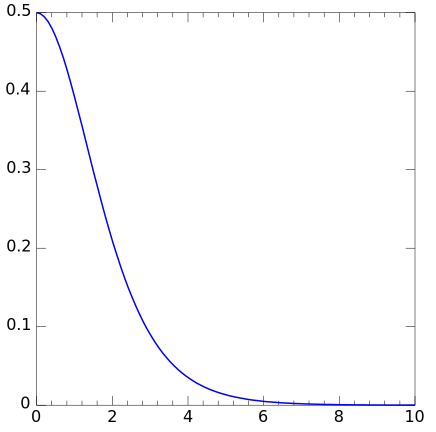
\includegraphics[width=0.6\textwidth]{images/Half-logistic distribution pdf.png}
        \caption{Probability density plots of half-logistic distribution}
    \end{figure}




% \begin{tabularx}{\textwidth}{l | X}
    {\color{darkblue} \textbf{$\mathcal{W}(X)$}:} {$k \in [0;\infty)\!$};\hspace{0.5cm}{\color{darkblue} \textbf{$\mathbb{E}[X]$}:} {$\log_e(4)=1.386\ldots$};\hspace{0.5cm}{\color{darkblue} \textbf{$Var[X]$}:} {$\pi^2/3-(\log_e(4))^2=1.368\ldots$};\hspace{0.5cm}\\{\color{darkblue} \textbf{$f_x$}:} {$\frac{2 e^{-k}}{(1+e^{-k})^2}\!$}{\color{darkblue} \textbf{$F_x$}:} {$\frac{1-e^{-k}}{1+e^{-k}}\!$}
% \end{tabularx}



    
        
\subsection{Fréchet distribution}


    \begin{figure}[H]
        \centering
        \includegraphics[width=0.6\textwidth]{images/Frechet pdf.png}
        \caption{PDF of the Fréchet distribution}
    \end{figure}




% \begin{tabularx}{\textwidth}{l | X}
    {\color{darkblue} \textbf{Params.}:} {$\alpha \in (0,\infty) $ shape. ,  (Optionally, two more parameters) ,  $ s \in (0,\infty) $ scale (default: $ s=1 \, $ ) ,  $  m \in (-\infty,\infty) $ location of minimum (default: $ m=0 \, $ )};\hspace{0.5cm}{\color{darkblue} \textbf{$\mathcal{W}(X)$}:} {$x>m$};\hspace{0.5cm}{\color{darkblue} \textbf{$\mathbb{E}[X]$}:} {$$\begin{cases}
                  \ m+s\Gamma\left(1-\frac{1}{\alpha}\right)  & \text{for } \alpha>1  \\
                  \ \infty              & \text{otherwise}
                \end{cases}$$};\hspace{0.5cm}{\color{darkblue} \textbf{$Var[X]$}:} {$$\begin{cases}
                  \ s^2\left(\Gamma\left(1-\frac{2}{\alpha}\right)- \left(\Gamma\left(1-\frac{1}{\alpha}\right)\right)^2\right)  & \text{for } \alpha>2  \\
                  \ \infty              & \text{otherwise}
                \end{cases}$$};\hspace{0.5cm}\\{\color{darkblue} \textbf{$f_x$}:} {$\frac{\alpha}{s} \; \left(\frac{x-m}{s}\right)^{-1-\alpha} \; e^{-(\frac{x-m}{s})^{-\alpha}}$}{\color{darkblue} \textbf{$F_x$}:} {$e^{-(\frac{x-m}{s})^{-\alpha}}$}
% \end{tabularx}



    
        
\subsection{Gompertz distribution}


    \begin{figure}[H]
        \centering
        \includegraphics[width=0.6\textwidth]{images/GompertzPDF.png}
        \caption{325px}
    \end{figure}




% \begin{tabularx}{\textwidth}{l | X}
    {\color{darkblue} \textbf{Params.}:} {shape $\eta>0\,\!$ , scale $b > 0\,\!$};\hspace{0.5cm}{\color{darkblue} \textbf{$\mathcal{W}(X)$}:} {$x \in [0, \infty)\!$};\hspace{0.5cm}{\color{darkblue} \textbf{$\mathbb{E}[X]$}:} {$(1/b)e^{\eta}\text{Ei}\left(-\eta\right)$ ,  $ \text {where  Ei}\left(z\right)=\int\limits_{-z}^{\infin}\left(e^{-v}/v\right)dv$};\hspace{0.5cm}{\color{darkblue} \textbf{$Var[X]$}:} {$\left(1/b\right)^2 e^{\eta}\{-2\eta { \ }_3\text {F}_3 \left(1,1,1;2,2,2;-\eta\right)+\gamma^2$ $$+\left(\pi^2/6\right)+2\gamma\ln\left(\eta\right)+[\ln\left(\eta\right)]^2-e^{\eta}[\text{Ei}\left(-\eta \right)]^2\}$$ ,  \begin{align}\text{ where } &\gamma \text{ is the Euler constant: }\,\!\\ &\gamma=-\psi\left(1\right)=\text{0.577215... }\end{align} \begin{align}\text { and } { }_3\text {F}_3&\left(1,1,1;2,2,2;-z\right)=\\&\sum_{k=0}^\infty\left[1/\left(k+1\right)^3\right]\left(-1\right)^k\left(z^k/k!\right)\end{align}};\hspace{0.5cm}\\{\color{darkblue} \textbf{$f_x$}:} {$b\eta \exp\left(\eta + bx -\eta e^{bx} \right)$}{\color{darkblue} \textbf{$F_x$}:} {$1-\exp\left(-\eta\left(e^{bx}-1 \right)\right)$}
% \end{tabularx}



    
        
\subsection{Lévy distribution}


    \begin{figure}[H]
        \centering
        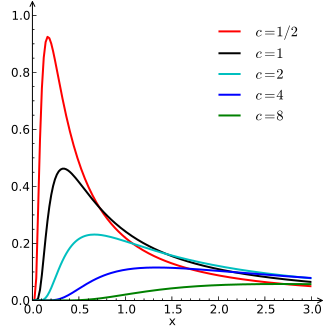
\includegraphics[width=0.6\textwidth]{images/Levy0 distributionPDF.png}
        \caption{Levy distribution PDF}
    \end{figure}




% \begin{tabularx}{\textwidth}{l | X}
    {\color{darkblue} \textbf{Params.}:} {$\mu$ location; $c > 0\,$ scale};\hspace{0.5cm}{\color{darkblue} \textbf{$\mathcal{W}(X)$}:} {$x \in [\mu, \infty)$};\hspace{0.5cm}{\color{darkblue} \textbf{$\mathbb{E}[X]$}:} {$\infty$};\hspace{0.5cm}{\color{darkblue} \textbf{$Var[X]$}:} {$\infty$};\hspace{0.5cm}\\{\color{darkblue} \textbf{$f_x$}:} {$\sqrt{\frac{c}{2\pi}}~~\frac{e^{-\frac{c}{2(x-\mu)}}}{(x-\mu)^{3/2}}$}{\color{darkblue} \textbf{$F_x$}:} {$\textrm{erfc}\left(\sqrt{\frac{c}{2(x-\mu)}}\right)$}
% \end{tabularx}



    
        
\subsection{Pareto distribution}


    \begin{figure}[H]
        \centering
        \includegraphics[width=0.6\textwidth]{images/Probability density function of Pareto distribution.png}
        \caption{Pareto Type I probability density functions for various \textit{α}}
    \end{figure}




% \begin{tabularx}{\textwidth}{l | X}
    {\color{darkblue} \textbf{Params.}:} {$x_\mathrm{m} > 0$ scale (real),  $\alpha > 0$ shape (real)};\hspace{0.5cm}{\color{darkblue} \textbf{$\mathcal{W}(X)$}:} {$x \in [x_\mathrm{m}, \infty)$};\hspace{0.5cm}{\color{darkblue} \textbf{$\mathbb{E}[X]$}:} {$$\begin{cases}
     \infty & \text{for }\alpha\le 1 \\
     \dfrac{\alpha x_\mathrm{m}}{\alpha-1} & \text{for }\alpha>1
   \end{cases}$$};\hspace{0.5cm}{\color{darkblue} \textbf{$Var[X]$}:} {$$\begin{cases}
     \infty & \text{for }\alpha\le 2 \\
     \dfrac{x_\mathrm{m}^2\alpha}{(\alpha-1)^2(\alpha-2)} & \text{for }\alpha>2
   \end{cases}$$};\hspace{0.5cm}\\{\color{darkblue} \textbf{$f_x$}:} {$\frac{\alpha x_\mathrm{m}^\alpha}{x^{\alpha+1}}$}{\color{darkblue} \textbf{$F_x$}:} {$1-\left(\frac{x_\mathrm{m}}{x}\right)^\alpha$}
% \end{tabularx}



    
        
\subsection{Nakagami distribution}


    \begin{figure}[H]
        \centering
        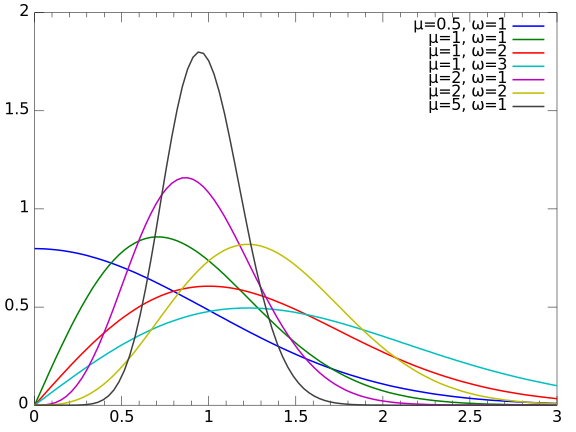
\includegraphics[width=0.6\textwidth]{images/Nakagami pdf.png}
        \caption{325px}
    \end{figure}




% \begin{tabularx}{\textwidth}{l | X}
    {\color{darkblue} \textbf{Params.}:} {$ m\text{ or } \mu \geq 0.5$ shape (real),  $\Omega \text{ or } \omega > 0$ spread (real)};\hspace{0.5cm}{\color{darkblue} \textbf{$\mathcal{W}(X)$}:} {$x > 0\!$};\hspace{0.5cm}{\color{darkblue} \textbf{$\mathbb{E}[X]$}:} {$\frac{\Gamma(m+\frac{1}{2})}{\Gamma(m)}\left(\frac{\Omega}{m}\right)^{1/2}$};\hspace{0.5cm}{\color{darkblue} \textbf{$Var[X]$}:} {$\Omega\left(1-\frac{1}{m}\left(\frac{\Gamma(m+\frac{1}{2})}{\Gamma(m)}\right)^2\right)$};\hspace{0.5cm}\\{\color{darkblue} \textbf{$f_x$}:} {$\frac{2m^m}{\Gamma(m)\Omega^m} x^{2m-1} \exp\left(-\frac{m}{\Omega}x^2 \right)$}{\color{darkblue} \textbf{$F_x$}:} {$\frac{\gamma \left(m,\frac{m}{\Omega} x^2\right)}{\Gamma(m)}$}
% \end{tabularx}



    
        
\subsection{Exponential distribution}


    \begin{figure}[H]
        \centering
        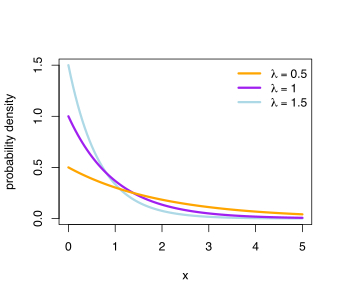
\includegraphics[width=0.6\textwidth]{images/Exponential probability density.png}
        \caption{plot of the probability density function of the exponential distribution}
    \end{figure}




% \begin{tabularx}{\textwidth}{l | X}
    {\color{darkblue} \textbf{Params.}:} {$\lambda > 0,$ rate, or inverse scale};\hspace{0.5cm}{\color{darkblue} \textbf{$\mathcal{W}(X)$}:} {$x \in [0, \infty)$};\hspace{0.5cm}{\color{darkblue} \textbf{$\mathbb{E}[X]$}:} {$\frac{1}{\lambda}$};\hspace{0.5cm}{\color{darkblue} \textbf{$Var[X]$}:} {$\frac{1}{\lambda^2}$};\hspace{0.5cm}\\{\color{darkblue} \textbf{$f_x$}:} {$\lambda e^{-\lambda x}$}{\color{darkblue} \textbf{$F_x$}:} {$1 - e^{-\lambda x}$}
% \end{tabularx}



    
        
\subsection{Erlang distribution}


    \begin{figure}[H]
        \centering
        \includegraphics[width=0.6\textwidth]{images/Erlang_dist_pdf.png}
        \caption{Probability density plots of Erlang distributions}
    \end{figure}




% \begin{tabularx}{\textwidth}{l | X}
    {\color{darkblue} \textbf{Params.}:} {$ k \in \{1,2,3,\ldots\},$ shape ,  $ \lambda \in (0,\infty),$ rate , alt.: $ \mu = 1/\lambda,$ scale};\hspace{0.5cm}{\color{darkblue} \textbf{$\mathcal{W}(X)$}:} {$ x \in [0, \infty)$};\hspace{0.5cm}{\color{darkblue} \textbf{$\mathbb{E}[X]$}:} {$ \frac{k}{\lambda}$};\hspace{0.5cm}{\color{darkblue} \textbf{$Var[X]$}:} {$ \frac{k}{\lambda^2}$};\hspace{0.5cm}\\{\color{darkblue} \textbf{$f_x$}:} {$ \frac{\lambda^k x^{k-1} e^{-\lambda x}}{(k-1)!}$}{\color{darkblue} \textbf{$F_x$}:} {$ P(k, \lambda x) = \frac{\gamma(k, \lambda x)}{(k - 1)!} = 1 - \sum_{n=0}^{k-1}\frac{1}{n!}e^{-\lambda x}(\lambda x)^{n}$}
% \end{tabularx}



    
        
\subsection{Shifted Gompertz distribution}


    \begin{figure}[H]
        \centering
        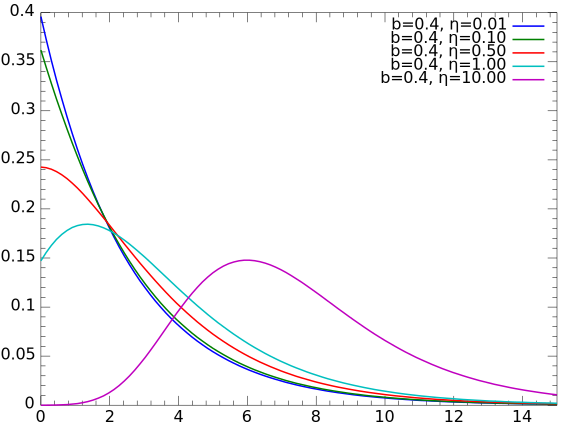
\includegraphics[width=0.6\textwidth]{images/Shiftedgompertz distribution PDF.png}
        \caption{Probability density plots of shifted Gompertz distributions}
    \end{figure}




% \begin{tabularx}{\textwidth}{l | X}
    {\color{darkblue} \textbf{Params.}:} {$b \geq 0$ scale (real),  $\eta\geq 0$ shape (real)};\hspace{0.5cm}{\color{darkblue} \textbf{$\mathcal{W}(X)$}:} {$x \in [0, \infty)\!$};\hspace{0.5cm}{\color{darkblue} \textbf{$\mathbb{E}[X]$}:} {$(-1/b)\{\mathrm{E}[\ln(X)] - \ln(\eta)\}\,$ where $X = \eta e^{-bx}\,$ and \begin{align}\mathrm{E}[\ln(X)] =& [1 {+} 1 / \eta]\!\!\int_0^\eta \!\!\!\! e^{-X}[\ln(X)]dX\\ &- 1/\eta\!\! \int_0^\eta \!\!\!\! X e^{-X}[\ln(X)] dX \end{align}};\hspace{0.5cm}{\color{darkblue} \textbf{$Var[X]$}:} {$(1/b^2)(\mathrm{E}\{[\ln(X)]^2\} - (\mathrm{E}[\ln(X)])^2)\,$ where $X = \eta e^{-bx}\,$ and \begin{align}\mathrm{E}\{[\ln(X)]^2\} =& [1 {+} 1 / \eta]\!\!\int_0^\eta \!\!\!\! e^{-X}[\ln(X)]^2 dX\\ &- 1/\eta \!\!\int_0^\eta \!\!\!\! X e^{-X}[\ln(X)]^2 dX \end{align}};\hspace{0.5cm}\\{\color{darkblue} \textbf{$f_x$}:} {$b e^{-bx} e^{-\eta e^{-bx}}\left[1 + \eta\left(1 - e^{-bx}\right)\right]$}{\color{darkblue} \textbf{$F_x$}:} {$\left(1 - e^{-bx}\right)e^{-\eta e^{-bx}}$}
% \end{tabularx}



    
        
\subsection{Gompertz distribution}


    \begin{figure}[H]
        \centering
        \includegraphics[width=0.6\textwidth]{images/GompertzPDF.png}
        \caption{325px}
    \end{figure}




% \begin{tabularx}{\textwidth}{l | X}
    {\color{darkblue} \textbf{Params.}:} {shape $\eta>0\,\!$ , scale $b > 0\,\!$};\hspace{0.5cm}{\color{darkblue} \textbf{$\mathcal{W}(X)$}:} {$x \in [0, \infty)\!$};\hspace{0.5cm}{\color{darkblue} \textbf{$\mathbb{E}[X]$}:} {$(1/b)e^{\eta}\text{Ei}\left(-\eta\right)$ ,  $ \text {where  Ei}\left(z\right)=\int\limits_{-z}^{\infin}\left(e^{-v}/v\right)dv$};\hspace{0.5cm}{\color{darkblue} \textbf{$Var[X]$}:} {$\left(1/b\right)^2 e^{\eta}\{-2\eta { \ }_3\text {F}_3 \left(1,1,1;2,2,2;-\eta\right)+\gamma^2$ $$+\left(\pi^2/6\right)+2\gamma\ln\left(\eta\right)+[\ln\left(\eta\right)]^2-e^{\eta}[\text{Ei}\left(-\eta \right)]^2\}$$ ,  \begin{align}\text{ where } &\gamma \text{ is the Euler constant: }\,\!\\ &\gamma=-\psi\left(1\right)=\text{0.577215... }\end{align} \begin{align}\text { and } { }_3\text {F}_3&\left(1,1,1;2,2,2;-z\right)=\\&\sum_{k=0}^\infty\left[1/\left(k+1\right)^3\right]\left(-1\right)^k\left(z^k/k!\right)\end{align}};\hspace{0.5cm}\\{\color{darkblue} \textbf{$f_x$}:} {$b\eta \exp\left(\eta + bx -\eta e^{bx} \right)$}{\color{darkblue} \textbf{$F_x$}:} {$1-\exp\left(-\eta\left(e^{bx}-1 \right)\right)$}
% \end{tabularx}



    
        
\subsection{Inverse Gaussian distribution}


    \begin{figure}[H]
        \centering
        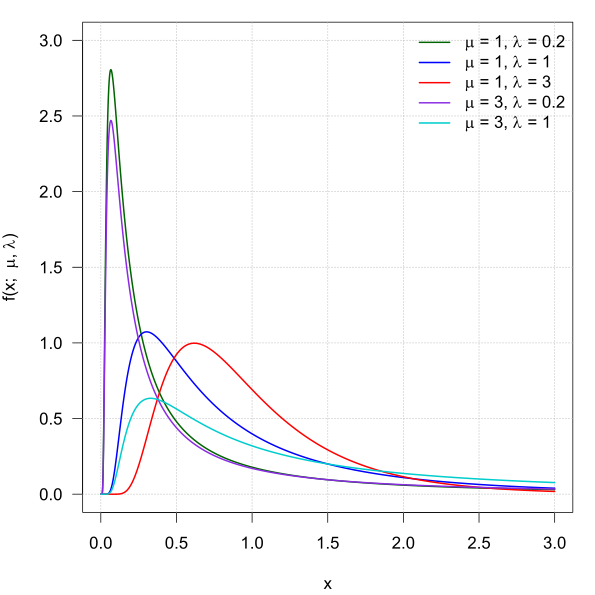
\includegraphics[width=0.6\textwidth]{images/Inverse Gaussian Probability Densitiy Function.png}
        \caption{325px}
    \end{figure}




% \begin{tabularx}{\textwidth}{l | X}
    {\color{darkblue} \textbf{Params.}:} {$\mu > 0$ ,  $\lambda > 0$};\hspace{0.5cm}{\color{darkblue} \textbf{Not.}:} {$\operatorname{IG}\left(\mu, \lambda\right)$};\hspace{0.5cm}{\color{darkblue} \textbf{$\mathcal{W}(X)$}:} {$ x \in (0,\infty)$};\hspace{0.5cm}{\color{darkblue} \textbf{$\mathbb{E}[X]$}:} {$\operatorname{E}[X] = \mu $ ,  $\operatorname{E}[\frac{1}{X}] = \frac{1}{\mu} + \frac{1}{\lambda}$};\hspace{0.5cm}{\color{darkblue} \textbf{$Var[X]$}:} {$\operatorname{Var}[ X] = \frac{\mu^3}{\lambda} $ ,  $\operatorname{Var}[\frac{1}{X}] = \frac{1}{\mu \lambda} + \frac{2}{\lambda^2}$};\hspace{0.5cm}\\{\color{darkblue} \textbf{$f_x$}:} {$ \sqrt\frac{\lambda}{2 \pi x^3} \exp\left[-\frac{\lambda (x-\mu)^2}{2 \mu^2 x}\right]$}{\color{darkblue} \textbf{$F_x$}:} {$ \Phi\left(\sqrt{\frac{\lambda}{x}} \left(\frac{x}{\mu}-1 \right)\right) $  ${}+\exp\left(\frac{2 \lambda}{\mu}\right) \Phi\left(-\sqrt{\frac{\lambda}{x}}\left(\frac{x}{\mu}+1 \right)\right)  $ where $ \Phi $ is the standard normal (standard Gaussian) distribution c.d.f.}
% \end{tabularx}



    
        
\subsection{Rayleigh distribution}


    \begin{figure}[H]
        \centering
        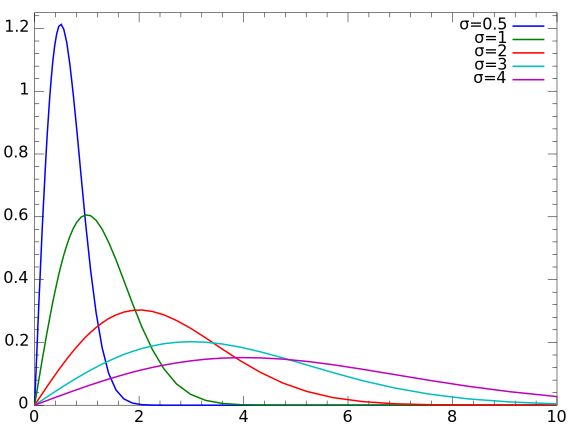
\includegraphics[width=0.6\textwidth]{images/Rayleigh distributionPDF.png}
        \caption{Plot of the Rayleigh PDF}
    \end{figure}




% \begin{tabularx}{\textwidth}{l | X}
    {\color{darkblue} \textbf{Params.}:} {scale: $\sigma>0$};\hspace{0.5cm}{\color{darkblue} \textbf{$\mathcal{W}(X)$}:} {$x\in [0,\infty)$};\hspace{0.5cm}{\color{darkblue} \textbf{$\mathbb{E}[X]$}:} {$\sigma \sqrt{\frac{\pi}{2}}$};\hspace{0.5cm}{\color{darkblue} \textbf{$Var[X]$}:} {$\frac{4 - \pi}{2} \sigma^2$};\hspace{0.5cm}\\{\color{darkblue} \textbf{$f_x$}:} {$\frac{x}{\sigma^2} e^{-x^2/\left(2\sigma^2\right)}$}{\color{darkblue} \textbf{$F_x$}:} {$1 - e^{-x^2/\left(2\sigma^2\right)}$}
% \end{tabularx}



    
        
\subsection{Weibull distribution}


    \begin{figure}[H]
        \centering
        \includegraphics[width=0.6\textwidth]{images/Weibull PDF.png}
        \caption{Probability distribution function}
    \end{figure}




% \begin{tabularx}{\textwidth}{l | X}
    {\color{darkblue} \textbf{Params.}:} {$\lambda\in (0, +\infty)\,$ scale ,  $k\in (0, +\infty)\,$ shape};\hspace{0.5cm}{\color{darkblue} \textbf{$\mathcal{W}(X)$}:} {$x \in [0, +\infty)\,$};\hspace{0.5cm}{\color{darkblue} \textbf{$\mathbb{E}[X]$}:} {$\lambda \, \Gamma(1+1/k)\,$};\hspace{0.5cm}{\color{darkblue} \textbf{$Var[X]$}:} {$\lambda^2\left[\Gamma\left(1+\frac{2}{k}\right) - \left(\Gamma\left(1+\frac{1}{k}\right)\right)^2\right]\,$};\hspace{0.5cm}\\{\color{darkblue} \textbf{$f_x$}:} {$$f(x)=\begin{cases}
\frac{k}{\lambda}\left(\frac{x}{\lambda}\right)^{k-1}e^{-(x/\lambda)^k} & x\geq0\\
0 & x<0\end{cases}$$}{\color{darkblue} \textbf{$F_x$}:} {$\begin{cases}1- e^{-(x/\lambda)^k} & x\geq0\\ 0 & x<0\end{cases}$}
% \end{tabularx}



    
        
\subsection{F-distribution}


    \begin{figure}[H]
        \centering
        \includegraphics[width=0.6\textwidth]{images/F-distribution pdf.png}
        \caption{325px}
    \end{figure}




% \begin{tabularx}{\textwidth}{l | X}
    {\color{darkblue} \textbf{Params.}:} {\textit{d}\textsubscript{1}, \textit{d}\textsubscript{2} > 0 deg. of freedom};\hspace{0.5cm}{\color{darkblue} \textbf{$\mathcal{W}(X)$}:} {$x \in (0, +\infty)\;$ if $d_1 = 1$ , otherwise $x \in [0, +\infty)\;$};\hspace{0.5cm}{\color{darkblue} \textbf{$\mathbb{E}[X]$}:} {$\frac{d_2}{d_2-2}\!$ ,  for \textit{d}\textsubscript{2} > 2};\hspace{0.5cm}{\color{darkblue} \textbf{$Var[X]$}:} {$\frac{2\,d_2^2\,(d_1+d_2-2)}{d_1 (d_2-2)^2 (d_2-4)}\!$ ,  for \textit{d}\textsubscript{2} > 4};\hspace{0.5cm}\\{\color{darkblue} \textbf{$f_x$}:} {$\frac{\sqrt{\frac{(d_1 x)^{d_1} d_2^{d_2}}{(d_1 x+d_2)^{d_1+d_2}}}}{x\,\mathrm{B}\!\left(\frac{d_1}{2},\frac{d_2}{2}\right)}\!$}{\color{darkblue} \textbf{$F_x$}:} {$I_{\frac{d_1 x}{d_1 x + d_2}} \left(\tfrac{d_1}{2}, \tfrac{d_2}{2} \right)$}
% \end{tabularx}



    
        
\subsection{Maxwell–Boltzmann distribution}


    \begin{figure}[H]
        \centering
        \includegraphics[width=0.6\textwidth]{images/Maxwell-Boltzmann distribution pdf.png}
        \caption{325px}
    \end{figure}




% \begin{tabularx}{\textwidth}{l | X}
    {\color{darkblue} \textbf{Params.}:} {$a>0$};\hspace{0.5cm}{\color{darkblue} \textbf{$\mathcal{W}(X)$}:} {$x\in (0;\infty)$};\hspace{0.5cm}{\color{darkblue} \textbf{$\mathbb{E}[X]$}:} {$\mu=2a \sqrt{\frac{2}{\pi}}$};\hspace{0.5cm}{\color{darkblue} \textbf{$Var[X]$}:} {$\sigma^2=\frac{a^2(3 \pi - 8)}{\pi}$};\hspace{0.5cm}\\{\color{darkblue} \textbf{$f_x$}:} {$\sqrt{\frac{2}{\pi}} \frac{x^2 e^{-x^2/\left(2a^2\right)}}{a^3}$}{\color{darkblue} \textbf{$F_x$}:} {$\operatorname{erf}\left(\frac{x}{\sqrt{2} a}\right) -\sqrt{\frac{2}{\pi}} \frac{x e^{-x^2/\left(2a^2\right)}}{a} $ where erf is the error function}
% \end{tabularx}



    


    \section{Continuous univariate supported on the whole real line}
        

        
    
        
\subsection{Variance-gamma distribution}





% \begin{tabularx}{\textwidth}{l | X}
    {\color{darkblue} \textbf{Params.}:} {$\mu$ location (real),  $\alpha$  (real),  $\beta$ asymmetry parameter (real),  $\lambda > 0$ ,  $\gamma = \sqrt{\alpha^2 - \beta^2} > 0 $};\hspace{0.5cm}{\color{darkblue} \textbf{$\mathcal{W}(X)$}:} {$x \in (-\infty; +\infty)\!$};\hspace{0.5cm}{\color{darkblue} \textbf{$\mathbb{E}[X]$}:} {$\mu + 2 \beta \lambda/ \gamma^2$};\hspace{0.5cm}{\color{darkblue} \textbf{$Var[X]$}:} {$2\lambda(1 + 2 \beta^2/\gamma^2)/\gamma^2$};\hspace{0.5cm}\\{\color{darkblue} \textbf{$f_x$}:} {$\frac{\gamma^{2\lambda} | x - \mu|^{\lambda-1/2} K_{\lambda-1/2} \left(\alpha|x - \mu|\right)}{\sqrt{\pi} \Gamma (\lambda)(2 \alpha)^{\lambda-1/2}} \; e^{\beta (x - \mu)}$ , ,  $K_\lambda$ denotes a modified Bessel function of the second kind,  $\Gamma$ denotes the Gamma function}
% \end{tabularx}



    
        
\subsection{Generalised hyperbolic distribution}





% \begin{tabularx}{\textwidth}{l | X}
    {\color{darkblue} \textbf{Params.}:} {$\lambda$  (real),  $\alpha$  (real),  $\beta$ asymmetry parameter (real),  $\delta$ scale parameter (real),  $\mu$ location (real),  $\gamma = \sqrt{\alpha^2 - \beta^2}$};\hspace{0.5cm}{\color{darkblue} \textbf{$\mathcal{W}(X)$}:} {$x \in (-\infty; +\infty)\!$};\hspace{0.5cm}{\color{darkblue} \textbf{$\mathbb{E}[X]$}:} {$\mu + \frac{\delta \beta K_{\lambda+1}(\delta \gamma)}{\gamma K_\lambda(\delta\gamma)}$};\hspace{0.5cm}{\color{darkblue} \textbf{$Var[X]$}:} {$$\frac{\delta K_{\lambda+1}(\delta \gamma)}{\gamma K_\lambda(\delta\gamma)} + \frac{\beta^2\delta^2}{\gamma^2}\left( \frac{K_{\lambda+2}(\delta\gamma)}{K_{\lambda}(\delta\gamma)} -
  \frac{K_{\lambda+1}^2(\delta\gamma)}{K_{\lambda}^2(\delta\gamma)} \right)$$};\hspace{0.5cm}\\{\color{darkblue} \textbf{$f_x$}:} {$\frac{(\gamma/\delta)^\lambda}{\sqrt{2\pi}K_\lambda(\delta \gamma)} \; e^{\beta (x - \mu)} \!$ ,  $\times \frac{K_{\lambda - 1/2}\left(\alpha \sqrt{\delta^2 + (x - \mu)^2}\right)}{\left(\sqrt{\delta^2 + (x - \mu)^2} / \alpha\right)^{1/2 - \lambda}} \!$}
% \end{tabularx}



    
        
\subsection{Normal-inverse Gaussian distribution}





% \begin{tabularx}{\textwidth}{l | X}
    {\color{darkblue} \textbf{Params.}:} {$\mu$ location (real),  $\alpha$ tail heaviness (real),  $\beta$ asymmetry parameter (real),  $\delta$ scale parameter (real),  $\gamma = \sqrt{\alpha^2 - \beta^2}$};\hspace{0.5cm}{\color{darkblue} \textbf{$\mathcal{W}(X)$}:} {$x \in (-\infty; +\infty)\!$};\hspace{0.5cm}{\color{darkblue} \textbf{$\mathbb{E}[X]$}:} {$\mu + \delta \beta / \gamma$};\hspace{0.5cm}{\color{darkblue} \textbf{$Var[X]$}:} {$\delta\alpha^2/\gamma^3$};\hspace{0.5cm}\\{\color{darkblue} \textbf{$f_x$}:} {$\frac{\alpha\delta K_1 \left(\alpha\sqrt{\delta^2 + (x - \mu)^2}\right)}{\pi \sqrt{\delta^2 + (x - \mu)^2}} \; e^{\delta \gamma + \beta (x - \mu)}$ , ,  $K_j$ denotes a modified Bessel function of the third kind}
% \end{tabularx}



    
        
\subsection{Holtsmark distribution}


    \begin{figure}[H]
        \centering
        \includegraphics[width=0.6\textwidth]{images/Levy distributionPDF.png}
        \caption{Symmetric stable distributions}
    \end{figure}




% \begin{tabularx}{\textwidth}{l | X}
    {\color{darkblue} \textbf{Params.}:} {\textit{c} ∈ (0, ∞) — scale parameter , 
\textit{μ} ∈ (−∞, ∞) — location parameter};\hspace{0.5cm}{\color{darkblue} \textbf{$\mathcal{W}(X)$}:} {\textit{x} ∈ \textbf{R}};\hspace{0.5cm}{\color{darkblue} \textbf{$\mathbb{E}[X]$}:} {\textit{μ}};\hspace{0.5cm}{\color{darkblue} \textbf{$Var[X]$}:} {infinite};\hspace{0.5cm}\\{\color{darkblue} \textbf{$f_x$}:} {expressible in terms of hypergeometric functions; see text}
% \end{tabularx}



    
        
\subsection{Asymmetric Laplace distribution}


    \begin{figure}[H]
        \centering
        \includegraphics[width=0.6\textwidth]{images/AsymmetricLaplace.jpg}
        \caption{350px}
    \end{figure}




% \begin{tabularx}{\textwidth}{l | X}
    {\color{darkblue} \textbf{Params.}:} {$m$ location (real),  $\lambda > 0$ scale (real),  $\kappa > 0$ asymmetry (real)};\hspace{0.5cm}{\color{darkblue} \textbf{$\mathcal{W}(X)$}:} {$x \in (-\infty; +\infty)\,$};\hspace{0.5cm}{\color{darkblue} \textbf{$\mathbb{E}[X]$}:} {$m+\frac{1-\kappa^2}{\lambda\kappa}$};\hspace{0.5cm}{\color{darkblue} \textbf{$Var[X]$}:} {$\frac{1+\kappa^4}{\lambda^2\kappa^2}$};\hspace{0.5cm}\\{\color{darkblue} \textbf{$f_x$}:} {(see article)}{\color{darkblue} \textbf{$F_x$}:} {(see article)}
% \end{tabularx}



    
        
\subsection{Johnson's SU-distribution}


    \begin{figure}[H]
        \centering
        \includegraphics[width=0.6\textwidth]{images/JohnsonSU.png}
        \caption{JohnsonSU}
    \end{figure}




% \begin{tabularx}{\textwidth}{l | X}
    {\color{darkblue} \textbf{Params.}:} {$ \gamma, \xi, \delta > 0, \lambda > 0 $ (real)};\hspace{0.5cm}{\color{darkblue} \textbf{$\mathcal{W}(X)$}:} {$ -\infty  \text{ to } +\infty $};\hspace{0.5cm}{\color{darkblue} \textbf{$\mathbb{E}[X]$}:} {$\xi - \lambda \exp \frac{\delta^{-2}}{2} \sinh\left(\frac{\gamma}{\delta}\right)$};\hspace{0.5cm}{\color{darkblue} \textbf{$Var[X]$}:} {$\frac{\lambda^2}{2} (\exp(\delta^{-2})-1) \left( \exp(\delta^{-2}) \cosh \left(\frac{2\gamma}{\delta} \right) +1 \right)$};\hspace{0.5cm}\\{\color{darkblue} \textbf{$f_x$}:} {$\frac{\delta}{\lambda\sqrt{2\pi}} \frac{1}{\sqrt{1 + \left(\frac{x-\xi}{\lambda}\right)^2}} e^{-\frac{1}{2}\left(\gamma+\delta \sinh^{-1} \left(\frac{x-\xi}{\lambda}\right)\right)^2}$}{\color{darkblue} \textbf{$F_x$}:} {$\Phi \left(\gamma + \delta \sinh^{-1} \left( \frac{x-\xi}{\lambda} \right) \right)$}
% \end{tabularx}



    
        
\subsection{Normal distribution}





% \begin{tabularx}{\textwidth}{l | X}
    {\color{darkblue} \textbf{Params.}:} {$\mu\in\R$ = mean (location),  $\sigma^2>0$ = variance (squared scale)};\hspace{0.5cm}{\color{darkblue} \textbf{Not.}:} {$\mathcal{N}(\mu,\sigma^2)$};\hspace{0.5cm}{\color{darkblue} \textbf{$\mathcal{W}(X)$}:} {$x\in\R$};\hspace{0.5cm}{\color{darkblue} \textbf{$\mathbb{E}[X]$}:} {$\mu$};\hspace{0.5cm}{\color{darkblue} \textbf{$Var[X]$}:} {$\sigma^2$};\hspace{0.5cm}\\{\color{darkblue} \textbf{$f_x$}:} {$\frac{1}{\sigma\sqrt{2\pi}} e^{-\frac{1}{2}\left(\frac{x - \mu}{\sigma}\right)^2}$}{\color{darkblue} \textbf{$F_x$}:} {$\frac{1}{2}\left[1 + \operatorname{erf}\left( \frac{x-\mu}{\sigma\sqrt{2}}\right)\right] $}
% \end{tabularx}



    
        
\subsection{Gumbel distribution}


    \begin{figure}[H]
        \centering
        \includegraphics[width=0.6\textwidth]{images/Gumbel-Density.png}
        \caption{Probability distribution function}
    \end{figure}




% \begin{tabularx}{\textwidth}{l | X}
    {\color{darkblue} \textbf{Params.}:} {$\mu,$ location (real),  $\beta>0,$ scale (real)};\hspace{0.5cm}{\color{darkblue} \textbf{$\mathcal{W}(X)$}:} {$x\in\mathbb{R}$};\hspace{0.5cm}{\color{darkblue} \textbf{$\mathbb{E}[X]$}:} {$\mu + \beta\gamma$ ,  where $\gamma$ is the Euler–Mascheroni constant};\hspace{0.5cm}{\color{darkblue} \textbf{$Var[X]$}:} {$\frac{\pi^2}{6}\beta^2$};\hspace{0.5cm}\\{\color{darkblue} \textbf{$f_x$}:} {$\frac{1}{\beta}e^{-(z+e^{-z})}$ ,  where $z=\frac{x-\mu}{\beta}$}{\color{darkblue} \textbf{$F_x$}:} {$e^{-e^{-(x-\mu)/\beta}}$}
% \end{tabularx}



    
        
\subsection{Fisher's z-distribution}


    \begin{figure}[H]
        \centering
        \includegraphics[width=0.6\textwidth]{images/FisherZDistriPDF.png}
        \caption{325px}
    \end{figure}




% \begin{tabularx}{\textwidth}{l | X}
    {\color{darkblue} \textbf{Params.}:} {$d_1>0,\ d_2>0$ deg. of freedom};\hspace{0.5cm}{\color{darkblue} \textbf{$\mathcal{W}(X)$}:} {$x \in (-\infty; +\infty)\!$};\hspace{0.5cm}\\{\color{darkblue} \textbf{$f_x$}:} {$\frac{2d_1^{d_1/2}d_2^{d_2/2}}{B(d_1/2,d_2/2)}\frac{e^{d_1x}}{\left(d_1e^{2x}+d_2\right)^{\left(d_1+d_2\right)/2}}\!$}
% \end{tabularx}



    
        
\subsection{Slash distribution}


    \begin{figure}[H]
        \centering
        \includegraphics[width=0.6\textwidth]{images/Slashpdf.png}
        \caption{center}
    \end{figure}




% \begin{tabularx}{\textwidth}{l | X}
    {\color{darkblue} \textbf{Params.}:} {none};\hspace{0.5cm}{\color{darkblue} \textbf{$\mathcal{W}(X)$}:} {$x\in(-\infty,\infty)$};\hspace{0.5cm}{\color{darkblue} \textbf{$\mathbb{E}[X]$}:} {Does not exist};\hspace{0.5cm}{\color{darkblue} \textbf{$Var[X]$}:} {Does not exist};\hspace{0.5cm}\\{\color{darkblue} \textbf{$f_x$}:} {$$\begin{cases}
\frac{\varphi(0) - \varphi(x)}{x^2} &  x \ne 0 \\
\frac{1}{2\sqrt{2\pi}} & x = 0 \\
\end{cases}$$}{\color{darkblue} \textbf{$F_x$}:} {$$\begin{cases}
\Phi(x) - \left[ \varphi(0) - \varphi(x) \right] / x &  x \ne 0 \\
1 / 2 & x = 0 \\
\end{cases}$$}
% \end{tabularx}



    
        
\subsection{Cauchy distribution}


    \begin{figure}[H]
        \centering
        \includegraphics[width=0.6\textwidth]{images/cauchy pdf.png}
        \caption{Probability density function for the Cauchy distribution}
    \end{figure}




% \begin{tabularx}{\textwidth}{l | X}
    {\color{darkblue} \textbf{Params.}:} {$x_0\!$ location (real),  $\gamma > 0$ scale (real)};\hspace{0.5cm}{\color{darkblue} \textbf{$\mathcal{W}(X)$}:} {$\displaystyle x \in (-\infty, +\infty)\!$};\hspace{0.5cm}{\color{darkblue} \textbf{$\mathbb{E}[X]$}:} {undefined};\hspace{0.5cm}{\color{darkblue} \textbf{$Var[X]$}:} {undefined};\hspace{0.5cm}\\{\color{darkblue} \textbf{$f_x$}:} {$\frac{1}{\pi\gamma\,\left[1 + \left(\frac{x-x_0}{\gamma}\right)^2\right]}\!$}{\color{darkblue} \textbf{$F_x$}:} {$\frac{1}{\pi} \arctan\left(\frac{x-x_0}{\gamma}\right)+\frac{1}{2}\!$}
% \end{tabularx}



    
        
\subsection{Skew normal distribution}


    \begin{figure}[H]
        \centering
        \includegraphics[width=0.6\textwidth]{images/Skew normal densities.png}
        \caption{Probability density plots of skew normal distributions}
    \end{figure}




% \begin{tabularx}{\textwidth}{l | X}
    {\color{darkblue} \textbf{Params.}:} {$\xi \,$ location (real),  $\omega \,$ scale (positive, real),  $\alpha \,$ shape (real)};\hspace{0.5cm}{\color{darkblue} \textbf{$\mathcal{W}(X)$}:} {$x \in (-\infty; +\infty)\!$};\hspace{0.5cm}{\color{darkblue} \textbf{$\mathbb{E}[X]$}:} {$\xi + \omega\delta\sqrt{\frac{2}{\pi}}$ where $\delta = \frac{\alpha}{\sqrt{1+\alpha^2}}$};\hspace{0.5cm}{\color{darkblue} \textbf{$Var[X]$}:} {$\omega^2\left(1 - \frac{2\delta^2}{\pi}\right)$};\hspace{0.5cm}\\{\color{darkblue} \textbf{$f_x$}:} {$\frac{2}{\omega \sqrt{2 \pi}} e^{-\frac{(x-\xi)^2}{2\omega^2}} \int_{-\infty}^{\alpha\left(\frac{x-\xi}{\omega}\right)} \frac{1}{\sqrt{2 \pi}}  e^{-\frac{t^2}{2}}\ dt$}{\color{darkblue} \textbf{$F_x$}:} {$\Phi\left(\frac{x-\xi}{\omega}\right)-2T\left(\frac{x-\xi}{\omega},\alpha\right)$ ,  $T(h,a)$ is Owen's T function}
% \end{tabularx}



    
        
\subsection{Hyperbolic secant distribution}


    \begin{figure}[H]
        \centering
        \includegraphics[width=0.6\textwidth]{images/Hyper_secant_pdf.png}
        \caption{Plot of the hyperbolic secant PDF}
    \end{figure}




% \begin{tabularx}{\textwidth}{l | X}
    {\color{darkblue} \textbf{Params.}:} {\textit{none}};\hspace{0.5cm}{\color{darkblue} \textbf{$\mathcal{W}(X)$}:} {$x \in (-\infty; +\infty)\!$};\hspace{0.5cm}{\color{darkblue} \textbf{$\mathbb{E}[X]$}:} {$0$};\hspace{0.5cm}{\color{darkblue} \textbf{$Var[X]$}:} {$1$};\hspace{0.5cm}\\{\color{darkblue} \textbf{$f_x$}:} {$\frac12 \; \operatorname{sech}\!\left(\frac{\pi}{2}\,x\right)\!$}{\color{darkblue} \textbf{$F_x$}:} {$\frac{2}{\pi} \arctan\!\left[\exp\!\left(\frac{\pi}{2}\,x\right)\right]\!$}
% \end{tabularx}



    
        
\subsection{Logistic distribution}


    \begin{figure}[H]
        \centering
        \includegraphics[width=0.6\textwidth]{images/Logisticpdfunction.png}
        \caption{Standard logistic PDF}
    \end{figure}




% \begin{tabularx}{\textwidth}{l | X}
    {\color{darkblue} \textbf{Params.}:} {$\mu,$ location (real),  $s > 0,$ scale (real)};\hspace{0.5cm}{\color{darkblue} \textbf{$\mathcal{W}(X)$}:} {$x \in (-\infty, \infty)$};\hspace{0.5cm}{\color{darkblue} \textbf{$\mathbb{E}[X]$}:} {$\mu$};\hspace{0.5cm}{\color{darkblue} \textbf{$Var[X]$}:} {$\frac{s^2 \pi^2}{3}$};\hspace{0.5cm}\\{\color{darkblue} \textbf{$f_x$}:} {$\frac{e^{-(x-\mu)/s}} {s\left(1+e^{-(x-\mu)/s}\right)^2}$}{\color{darkblue} \textbf{$F_x$}:} {$\frac{1}{1+e^{-(x-\mu)/s}}$}
% \end{tabularx}



    
        
\subsection{Noncentral t-distribution}


    \begin{figure}[H]
        \centering
        \includegraphics[width=0.6\textwidth]{images/nc student t pdf.png}
        \caption{325px}
    \end{figure}




% \begin{tabularx}{\textwidth}{l | X}
    {\color{darkblue} \textbf{Params.}:} {ν > 0 degrees of freedom,  $\mu \in \Re \,\!$ noncentrality parameter};\hspace{0.5cm}{\color{darkblue} \textbf{$\mathcal{W}(X)$}:} {$x \in (-\infty; +\infty)\,\!$};\hspace{0.5cm}{\color{darkblue} \textbf{$\mathbb{E}[X]$}:} {see text};\hspace{0.5cm}{\color{darkblue} \textbf{$Var[X]$}:} {see text};\hspace{0.5cm}\\{\color{darkblue} \textbf{$f_x$}:} {see text}
% \end{tabularx}



    
        
\subsection{Landau distribution}


    \begin{figure}[H]
        \centering
        \includegraphics[width=0.6\textwidth]{images/Landau Distribution PDF.png}
        \caption{350px}
    \end{figure}




% \begin{tabularx}{\textwidth}{l | X}
    {\color{darkblue} \textbf{Params.}:} {$c \in(0,\infty)$ — scale parameter ,  $\mu\in(-\infty,\infty)$ — location parameter};\hspace{0.5cm}{\color{darkblue} \textbf{$\mathcal{W}(X)$}:} {$\mathbb{R}$};\hspace{0.5cm}{\color{darkblue} \textbf{$\mathbb{E}[X]$}:} {Undefined};\hspace{0.5cm}{\color{darkblue} \textbf{$Var[X]$}:} {Undefined};\hspace{0.5cm}\\{\color{darkblue} \textbf{$f_x$}:} {$ \frac{1}{\pi c}\int_0^\infty e^{-t}\cos\left(t\left(\frac{x-\mu}{c}\right) + \frac{2t}{\pi}\log\left(\frac{t}{c}\right)\right)\, dt$}
% \end{tabularx}



    
        
\subsection{Generalized normal distribution}


    \begin{figure}[H]
        \centering
        \includegraphics[width=0.6\textwidth]{images/Generalized normal densities.png}
        \caption{Probability density plots of generalized normal distributions}
    \end{figure}




% \begin{tabularx}{\textwidth}{l | X}
    {\color{darkblue} \textbf{Params.}:} {$ \mu \,$ location (real),  $ \alpha \,$ scale (positive, real),  $ \beta \,$ shape (positive, real)};\hspace{0.5cm}{\color{darkblue} \textbf{$\mathcal{W}(X)$}:} {$x \in (-\infty; +\infty)\!$};\hspace{0.5cm}{\color{darkblue} \textbf{$\mathbb{E}[X]$}:} {$ \mu \,$};\hspace{0.5cm}{\color{darkblue} \textbf{$Var[X]$}:} {$\frac{\alpha^2\Gamma(3/\beta)}{\Gamma(1/\beta)}$};\hspace{0.5cm}\\{\color{darkblue} \textbf{$f_x$}:} {$\frac{\beta}{2\alpha\Gamma(1/\beta)} \; e^{-(|x-\mu|/\alpha)^\beta}$ , ,  $\Gamma$ denotes the gamma function}{\color{darkblue} \textbf{$F_x$}:} {$\frac{1}{2}+ \frac{\text{sign}(x - \mu)}{2} \frac{1}{\Gamma \left(\frac{1}{\beta}\right)} \gamma\left(\frac{1}{\beta}, x \alpha^\beta\right)$ .}
% \end{tabularx}



    
        
\subsection{Generalized normal distribution}


    \begin{figure}[H]
        \centering
        \includegraphics[width=0.6\textwidth]{images/Generalized normal densities.png}
        \caption{Probability density plots of generalized normal distributions}
    \end{figure}




% \begin{tabularx}{\textwidth}{l | X}
    {\color{darkblue} \textbf{Params.}:} {$ \mu \,$ location (real),  $ \alpha \,$ scale (positive, real),  $ \beta \,$ shape (positive, real)};\hspace{0.5cm}{\color{darkblue} \textbf{$\mathcal{W}(X)$}:} {$x \in (-\infty; +\infty)\!$};\hspace{0.5cm}{\color{darkblue} \textbf{$\mathbb{E}[X]$}:} {$ \mu \,$};\hspace{0.5cm}{\color{darkblue} \textbf{$Var[X]$}:} {$\frac{\alpha^2\Gamma(3/\beta)}{\Gamma(1/\beta)}$};\hspace{0.5cm}\\{\color{darkblue} \textbf{$f_x$}:} {$\frac{\beta}{2\alpha\Gamma(1/\beta)} \; e^{-(|x-\mu|/\alpha)^\beta}$ , ,  $\Gamma$ denotes the gamma function}{\color{darkblue} \textbf{$F_x$}:} {$\frac{1}{2}+ \frac{\text{sign}(x - \mu)}{2} \frac{1}{\Gamma \left(\frac{1}{\beta}\right)} \gamma\left(\frac{1}{\beta}, x \alpha^\beta\right)$ .}
% \end{tabularx}



    
        
\subsection{Student's t-distribution}


    \begin{figure}[H]
        \centering
        \includegraphics[width=0.6\textwidth]{images/student t pdf.png}
        \caption{325px}
    \end{figure}




% \begin{tabularx}{\textwidth}{l | X}
    {\color{darkblue} \textbf{Params.}:} {$\nu > 0$ degrees of freedom (real)};\hspace{0.5cm}{\color{darkblue} \textbf{$\mathcal{W}(X)$}:} {$x \in (- \infty, \infty)$};\hspace{0.5cm}{\color{darkblue} \textbf{$\mathbb{E}[X]$}:} {0 for $\nu > 1$ , otherwise undefined};\hspace{0.5cm}{\color{darkblue} \textbf{$Var[X]$}:} {$\textstyle\frac{\nu}{\nu-2}$ for $\nu > 2$ , ∞ for $1 < \nu \le 2$ , otherwise undefined};\hspace{0.5cm}\\{\color{darkblue} \textbf{$f_x$}:} {$\textstyle\frac{\Gamma \left(\frac{\nu+1}{2} \right)} {\sqrt{\nu\pi}\,\Gamma \left(\frac{\nu}{2} \right)} \left(1+\frac{x^2}{\nu} \right)^{-\frac{\nu+1}{2}}\!$}
% \end{tabularx}



    
        
\subsection{Laplace distribution}


    \begin{figure}[H]
        \centering
        \includegraphics[width=0.6\textwidth]{images/Laplace pdf mod.png}
        \caption{Probability density plots of Laplace distributions}
    \end{figure}




% \begin{tabularx}{\textwidth}{l | X}
    {\color{darkblue} \textbf{Params.}:} {$\mu$ location (real),  $b > 0$ scale (real)};\hspace{0.5cm}{\color{darkblue} \textbf{$\mathcal{W}(X)$}:} {$\mathbb{R}$};\hspace{0.5cm}{\color{darkblue} \textbf{$\mathbb{E}[X]$}:} {$\mu$};\hspace{0.5cm}{\color{darkblue} \textbf{$Var[X]$}:} {$2b^2$};\hspace{0.5cm}\\{\color{darkblue} \textbf{$f_x$}:} {$\frac{1}{2b} \exp \left(-\frac{|x-\mu|}b \right)$}{\color{darkblue} \textbf{$F_x$}:} {$$\begin{cases}
                \frac{1}{2} \exp \left( \frac{x-\mu}{b} \right) & \text{if }x \leq \mu \\[8pt]
                1-\frac{1}{2} \exp \left( -\frac{x-\mu}{b} \right) & \text{if }x \geq \mu
              \end{cases}$$}
% \end{tabularx}



    
        
\subsection{Voigt profile}


    \begin{figure}[H]
        \centering
        \includegraphics[width=0.6\textwidth]{images/VoigtPDF.png}
        \caption{Plot of the centered Voigt profile for four cases}
    \end{figure}




% \begin{tabularx}{\textwidth}{l | X}
    {\color{darkblue} \textbf{Params.}:} {$\gamma,\sigma>0$};\hspace{0.5cm}{\color{darkblue} \textbf{$\mathcal{W}(X)$}:} {$x\in(-\infty,\infty)$};\hspace{0.5cm}{\color{darkblue} \textbf{$\mathbb{E}[X]$}:} {(not defined)};\hspace{0.5cm}{\color{darkblue} \textbf{$Var[X]$}:} {(not defined)};\hspace{0.5cm}\\{\color{darkblue} \textbf{$f_x$}:} {$$\frac{\Re[w(z)]}{\sigma\sqrt{2\pi}},
              ~~~z=\frac{x+i\gamma}{\sigma\sqrt{2}}$$}{\color{darkblue} \textbf{$F_x$}:} {(complicated - see text)}
% \end{tabularx}



    


    \section{Continuous univariate with support whose type varies}
        

        
    
        
\subsection{Shifted log-logistic distribution}





% \begin{tabularx}{\textwidth}{l | X}
    {\color{darkblue} \textbf{Params.}:} {$\mu \in (-\infty,+\infty) \,$ location (real),  $\sigma \in (0,+\infty)    \,$ scale (real),  $\xi\in (-\infty,+\infty)  \,$ shape (real)};\hspace{0.5cm}{\color{darkblue} \textbf{$\mathcal{W}(X)$}:} {$x \geqslant \mu -\sigma/\xi\,\;(\xi > 0)$ ,  $x \leqslant \mu -\sigma/\xi\,\;(\xi < 0)$ ,  $x \in (-\infty, +\infty)   \,\;(\xi = 0)$};\hspace{0.5cm}{\color{darkblue} \textbf{$\mathbb{E}[X]$}:} {$\mu + \frac{\sigma}{\xi}(\alpha \csc(\alpha)-1)$ , 
where $\alpha= \pi \xi\, $};\hspace{0.5cm}{\color{darkblue} \textbf{$Var[X]$}:} {$ \frac{\sigma^2}{\xi^2}[2\alpha \csc(2 \alpha) - (\alpha \csc(\alpha))^2]  $ , 
where $\alpha= \pi \xi\, $};\hspace{0.5cm}\\{\color{darkblue} \textbf{$f_x$}:} {$\frac{(1+\xi z)^{-(1/\xi +1)}}{\sigma\left(1 + (1+\xi z)^{-1/\xi}\right)^2} $ , 
where $z=(x-\mu)/\sigma\,$}{\color{darkblue} \textbf{$F_x$}:} {$\left(1+(1 + \xi z)^{-1/\xi}\right)^{-1} \,$ , 
where $z=(x-\mu)/\sigma\,$}
% \end{tabularx}



    
        
\subsection{Generalized extreme value distribution}





% \begin{tabularx}{\textwidth}{l | X}
    {\color{darkblue} \textbf{Params.}:} {\textit{μ} ∈ \textbf{R} — location,,  \textit{σ} > 0 — scale,,  \textit{ξ} ∈ \textbf{R} — shape.};\hspace{0.5cm}{\color{darkblue} \textbf{Not.}:} {$\textrm{GEV}(\mu,\,\sigma,\,\xi)$};\hspace{0.5cm}{\color{darkblue} \textbf{$\mathcal{W}(X)$}:} {\textit{x} ∈ [ \textit{μ} − \textit{σ / ξ}, +∞)   when \textit{ξ} > 0,, \textit{x} ∈ (−∞, +∞)   when \textit{ξ} = 0,, \textit{x} ∈ (−∞, \textit{μ} − \textit{σ / ξ} ]   when \textit{ξ} < 0.};\hspace{0.5cm}{\color{darkblue} \textbf{$\mathbb{E}[X]$}:} {$\begin{cases}\mu + \sigma(g_1 - 1)/\xi & \text{if}\ \xi\neq 0,\xi<1,\\ \mu + \sigma\,\gamma & \text{if}\ \xi=0,\\ \infty & \text{if}\ \xi\geq 1,\end{cases}$ where \textit{g\textsubscript{k}} = Γ(1 − \textit{kξ}), ,  and $\gamma$ is Euler’s constant.};\hspace{0.5cm}{\color{darkblue} \textbf{$Var[X]$}:} {$\begin{cases}\sigma^2\,(g_2-g_1^2)/\xi^2 & \text{if}\ \xi\neq0,\xi<\frac12,\\ \sigma^2\,\frac{\pi^2}{6} & \text{if}\ \xi=0, \\ \infty & \text{if}\ \xi\geq\frac12,\end{cases}$ .};\hspace{0.5cm}\\{\color{darkblue} \textbf{$f_x$}:} {$\frac{1}{\sigma}\,t(x)^{\xi+1}e^{-t(x)},$   
where $t(x) = \begin{cases}\big(1+\xi(\tfrac{x-\mu}{\sigma})\big)^{-1/\xi} & \textrm{if}\ \xi\neq0 \\ e^{-(x-\mu)/\sigma} & \textrm{if}\ \xi=0\end{cases}$}{\color{darkblue} \textbf{$F_x$}:} {$e^{-t(x)},\,$   for \textit{x} ∈ support}
% \end{tabularx}



    
        
\subsection{Q-Weibull distribution}


    \begin{figure}[H]
        \centering
        \includegraphics[width=0.6\textwidth]{images/QWeibull pdf.png}
        \caption{Graph of the \textit{q}-Weibull pdf}
    \end{figure}




% \begin{tabularx}{\textwidth}{l | X}
    {\color{darkblue} \textbf{Params.}:} {$q < 2 $ shape (real) ,  $ \lambda > 0 $ rate (real) ,  $\kappa>0\,$ shape (real)};\hspace{0.5cm}{\color{darkblue} \textbf{$\mathcal{W}(X)$}:} {$x \in [0; +\infty)\! \text{ for }q \ge 1 $ ,  $ x \in [0; {\lambda \over {(1-q)^{1/\kappa}}}) \text{ for } q<1 $};\hspace{0.5cm}{\color{darkblue} \textbf{$\mathbb{E}[X]$}:} {(see article)};\hspace{0.5cm}\\{\color{darkblue} \textbf{$f_x$}:} {$$\begin{cases}
(2-q)\frac{\kappa}{\lambda}\left(\frac{x}{\lambda}\right)^{\kappa-1}e_{q}^{-(x/\lambda)^{\kappa}} & x\geq0\\
0 & x<0\end{cases}$$}{\color{darkblue} \textbf{$F_x$}:} {$\begin{cases}1- e_{q'}^{-(x/\lambda')^\kappa} & x\geq0\\ 0 & x<0\end{cases}$}
% \end{tabularx}



    
        
\subsection{Q-Gaussian distribution}


    \begin{figure}[H]
        \centering
        \includegraphics[width=0.6\textwidth]{images/The PDF of QGaussian.png}
        \caption{Probability density plots of \textit{q}-Gaussian distributions}
    \end{figure}




% \begin{tabularx}{\textwidth}{l | X}
    {\color{darkblue} \textbf{Params.}:} {$q < 3 $ shape (real) ,  $ \beta > 0 $ (real)};\hspace{0.5cm}{\color{darkblue} \textbf{$\mathcal{W}(X)$}:} {$x \in (-\infty; +\infty)\!$ for $1\le q < 3 $ ,  $x \in \left[\pm {1 \over \sqrt{\beta(1-q)}}\right] $ for $q < 1 $};\hspace{0.5cm}{\color{darkblue} \textbf{$\mathbb{E}[X]$}:} {$0\text{ for }q<2$ , otherwise undefined};\hspace{0.5cm}{\color{darkblue} \textbf{$Var[X]$}:} {$ { 1 \over {\beta (5-3q)}} \text{ for } q < {5 \over 3}$ ,  $$\infty \text{ for } {5 \over 3} \le q < 2$$ ,  $ \text{Undefined for }2 \le q <3$};\hspace{0.5cm}\\{\color{darkblue} \textbf{$f_x$}:} {${\sqrt{\beta} \over C_q} e_q({-\beta x^2}) $}
% \end{tabularx}



    
        
\subsection{Generalized chi-squared distribution}


    \begin{figure}[H]
        \centering
        \includegraphics[width=0.6\textwidth]{images/Generalized chi-square PDF.png}
        \caption{Generalized chi-square probability density function}
    \end{figure}




% \begin{tabularx}{\textwidth}{l | X}
    {\color{darkblue} \textbf{Params.}:} {$\boldsymbol{\lambda}$ , vector of weights of chi-square components,  $\boldsymbol{m}$ , vector of degrees of freedom of chi-square components,  $\boldsymbol{\delta}$ , vector of non-centrality parameters of chi-square components,  $\sigma$ , scale of normal term};\hspace{0.5cm}{\color{darkblue} \textbf{$\mathcal{W}(X)$}:} {$x\in\R$};\hspace{0.5cm}{\color{darkblue} \textbf{$\mathbb{E}[X]$}:} {$\sum \lambda_j (m_j+\delta_j^2)$};\hspace{0.5cm}{\color{darkblue} \textbf{$Var[X]$}:} {$2 \sum \lambda_j^2 (m_j+2 \delta_j^2) + \sigma^2$};\hspace{0.5cm}\\
% \end{tabularx}



    
        
\subsection{Tukey lambda distribution}


    \begin{figure}[H]
        \centering
        \includegraphics[width=0.6\textwidth]{images/Several samples of the pdfs of the Tukey lambda distributions.png}
        \caption{Probability density plots of Tukey lambda distributions}
    \end{figure}




% \begin{tabularx}{\textwidth}{l | X}
    {\color{darkblue} \textbf{Params.}:} {\textit{λ} ∈ \textbf{R} — shape parameter};\hspace{0.5cm}{\color{darkblue} \textbf{Not.}:} {Tukey(\textit{λ})};\hspace{0.5cm}{\color{darkblue} \textbf{$\mathcal{W}(X)$}:} {\textit{x} ∈ [−1/\textit{λ}, 1/\textit{λ}] for \textit{λ} > 0,, \textit{x} ∈ \textbf{R} for \textit{λ} ≤ 0};\hspace{0.5cm}{\color{darkblue} \textbf{$\mathbb{E}[X]$}:} {$0,\,\,\lambda > -1$};\hspace{0.5cm}{\color{darkblue} \textbf{$Var[X]$}:} {$\frac{2}{\lambda^2}\bigg(\frac{1}{1+2\lambda}-\frac{\Gamma(\lambda+1)^2}{\Gamma(2\lambda+2)}\bigg),\,\,\lambda > -1/2$ ,  $\frac{ \pi^{2} }{ 3 },\,\,\lambda\,=\,0$};\hspace{0.5cm}\\{\color{darkblue} \textbf{$f_x$}:} {$(Q(p;\lambda),q(p;\lambda)^{-1}),\, 0\leq\,p\,\leq\,1$}{\color{darkblue} \textbf{$F_x$}:} {$(e^{-x}+1)^{-1},\,\,\lambda\,=\,0\,$ (special case),  $(Q(p;\lambda),p),\, 0\leq\,p\,\leq\,1\,$ (general case)}
% \end{tabularx}



    
        
\subsection{Generalized Pareto distribution}


    \begin{figure}[H]
        \centering
        \includegraphics[width=0.6\textwidth]{images/Gpdpdf.png}
        \caption{Gpdpdf}
    \end{figure}




% \begin{tabularx}{\textwidth}{l | X}
    {\color{darkblue} \textbf{Params.}:} {$\mu \in (-\infty,\infty) \,$ location (real),  $\sigma \in (0,\infty)    \,$ scale (real),  $\xi\in (-\infty,\infty)  \,$ shape (real)};\hspace{0.5cm}{\color{darkblue} \textbf{$\mathcal{W}(X)$}:} {$x \geqslant \mu\,\;(\xi \geqslant 0)$ ,  $\mu \leqslant x \leqslant \mu-\sigma/\xi\,\;(\xi < 0)$};\hspace{0.5cm}{\color{darkblue} \textbf{$\mathbb{E}[X]$}:} {$\mu + \frac{\sigma}{1-\xi}\, \; (\xi < 1) $};\hspace{0.5cm}{\color{darkblue} \textbf{$Var[X]$}:} {$\frac{\sigma^2}{(1-\xi)^2(1-2\xi)}\, \; (\xi < 1/2)$};\hspace{0.5cm}\\{\color{darkblue} \textbf{$f_x$}:} {$\frac{1}{\sigma}(1 + \xi z )^{-(1/\xi +1)} $ , 
where $z=\frac{x-\mu}{\sigma}$}{\color{darkblue} \textbf{$F_x$}:} {$1-(1+\xi z)^{-1/\xi} \,$}
% \end{tabularx}



    
        
\subsection{Q-exponential distribution}


    \begin{figure}[H]
        \centering
        \includegraphics[width=0.6\textwidth]{images/The Probability Density Function of q-exponential distribution.png}
        \caption{Probability density plots of \textit{q}-exponential distributions}
    \end{figure}




% \begin{tabularx}{\textwidth}{l | X}
    {\color{darkblue} \textbf{Params.}:} {$q < 2 $ shape (real) ,  $ \lambda > 0 $ rate (real)};\hspace{0.5cm}{\color{darkblue} \textbf{$\mathcal{W}(X)$}:} {$x \in [0, \infty) \text{ for } q \ge 1 $ ,  $ x \in \left[0, \frac{1}{\lambda(1-q)}\right) \text{ for } q<1 $};\hspace{0.5cm}{\color{darkblue} \textbf{$\mathbb{E}[X]$}:} {$\frac{1}{\lambda (3-2q)} \text{ for } q < \frac{3}{2} $ ,  Otherwise undefined};\hspace{0.5cm}{\color{darkblue} \textbf{$Var[X]$}:} {$\frac{q-2}{(2q-3)^2 (3q-4) \lambda^2} \text{ for } q < \frac{4}{3}$};\hspace{0.5cm}\\{\color{darkblue} \textbf{$f_x$}:} {$(2-q) \lambda e_q^{-\lambda x} $}{\color{darkblue} \textbf{$F_x$}:} {$1-e_{q'}^{-\lambda x / q'} \text{ where } q' = \frac{1}{2-q}$}
% \end{tabularx}



    


    \section{Mixed continuous-discrete univariate }
        

        
    


    \section{Multivariate (joint)}
        
            \subsection{Discrete}

            
    
        
\subsubsection{Negative multinomial distribution}





% \begin{tabularx}{\textwidth}{l | X}
    {\color{darkblue} \textbf{Params.}:} {\textit{x}\textsubscript{0} ∈ \textbf{N}\textsubscript{0} — the number of failures before the experiment is stopped,, \textit{p} ∈ \textbf{R}\textsuperscript{\textit{m}} — \textit{m}-vector of "success" probabilities,, <hr>\textit{p}\textsubscript{0} = 1 − (\textit{p}\textsubscript{1}+…+\textit{p}\textsubscript{\textit{m}}) — the probability of a "failure".};\hspace{0.5cm}{\color{darkblue} \textbf{Not.}:} {$\textrm{NM}(x_0,\,p)$};\hspace{0.5cm}{\color{darkblue} \textbf{$\mathcal{W}(X)$}:} {$x_i \in \{0,1,2,\ldots\}, 1\leq i\leq m$};\hspace{0.5cm}{\color{darkblue} \textbf{$\mathbb{E}[X]$}:} {$ \tfrac{x_0}{p_0}\,p $};\hspace{0.5cm}{\color{darkblue} \textbf{$Var[X]$}:} {$ \tfrac{x_0}{p_0^2}\,pp' + \tfrac{x_0}{p_0}\,\operatorname{diag}(p) $};\hspace{0.5cm}\\{\color{darkblue} \textbf{$f_x$}:} {$\Gamma\!\left(\sum_{i=0}^m{x_i}\right)\frac{p_0^{x_0}}{\Gamma(x_0)} \prod_{i=1}^m{\frac{p_i^{x_i}}{x_i!}},$ ,  where Γ(\textit{x}) is the Gamma function.}
% \end{tabularx}



    
        
\subsubsection{Multinomial distribution}





% \begin{tabularx}{\textwidth}{l | X}
    {\color{darkblue} \textbf{Params.}:} {$n > 0$ number of trials (integer),  $p_1, \ldots, p_k$ event probabilities ( $\Sigma p_i = 1$ )};\hspace{0.5cm}{\color{darkblue} \textbf{$\mathcal{W}(X)$}:} {$x_i \in \{0, \dots, n\}, \,\,\,\,i \in \{1,\dots,k\}$ ,  $\Sigma x_i = n\!$};\hspace{0.5cm}{\color{darkblue} \textbf{$\mathbb{E}[X]$}:} {$\operatorname E(X_i) = np_i$};\hspace{0.5cm}{\color{darkblue} \textbf{$Var[X]$}:} {$\operatorname{Var}(X_i) = n p_i (1-p_i)$ ,  $\operatorname{Cov}(X_i,X_j) = - n p_i p_j~~(i\neq j)$};\hspace{0.5cm}\\{\color{darkblue} \textbf{$f_x$}:} {$\frac{n!}{x_1!\cdots x_k!} p_1^{x_1} \cdots p_k^{x_k}$}
% \end{tabularx}



    
        
\subsubsection{Dirichlet-multinomial distribution}





% \begin{tabularx}{\textwidth}{l | X}
    {\color{darkblue} \textbf{Params.}:} {$n > 0$ number of trials (positive integer),  $\alpha_1, \ldots, \alpha_{K}>0$};\hspace{0.5cm}{\color{darkblue} \textbf{$\mathcal{W}(X)$}:} {$x_i \in \{0,\dots,n\}$ ,  $\Sigma x_i = n\!$};\hspace{0.5cm}{\color{darkblue} \textbf{$\mathbb{E}[X]$}:} {$E(X_i) = n\frac{\alpha_i}{\sum \alpha_k}$};\hspace{0.5cm}{\color{darkblue} \textbf{$Var[X]$}:} {$Var(X_i) = n\frac{\alpha_i}{\sum \alpha_k}\left(1-\frac{\alpha_i}{\sum \alpha_k}\right)\left(\frac{n+\sum \alpha_k}{1+\sum \alpha_k}\right)$ ,  $\textstyle {\mathrm{Cov}}(X_i,X_j) = - n \frac{\alpha_i \alpha_j}{(\sum \alpha_k)^2} \left(\frac{n+\sum \alpha_k}{1+\sum \alpha_k}\right)~~(i\neq j)$};\hspace{0.5cm}\\{\color{darkblue} \textbf{$f_x$}:} {$$\frac{\left(n!\right)\Gamma\left(\sum \alpha_k\right)}
{\Gamma\left(n+\sum \alpha_k\right)}\prod_{k=1}^K\frac{\Gamma(x_{k}+\alpha_{k})}{\left(x_{k}!\right)\Gamma(\alpha_{k})}$$}
% \end{tabularx}



    

        
            \subsection{Continuous}

            
    
        
\subsubsection{Multivariate Laplace distribution}





% \begin{tabularx}{\textwidth}{l | X}
    {\color{darkblue} \textbf{Params.}:} {\textbf{\textit{μ}} ∈ \textbf{R}\textsuperscript{\textit{k}} — location, \textbf{Σ} ∈ \textbf{R}\textsuperscript{\textit{k×k}} — covariance (positive-definite matrix)};\hspace{0.5cm}{\color{darkblue} \textbf{$\mathcal{W}(X)$}:} {\textbf{\textit{x}} ∈ \textbf{μ} + span(\textbf{Σ}) ⊆ \textbf{R}\textsuperscript{\textit{k}}};\hspace{0.5cm}{\color{darkblue} \textbf{$\mathbb{E}[X]$}:} {\textbf{\textit{μ}}};\hspace{0.5cm}{\color{darkblue} \textbf{$Var[X]$}:} {\textbf{Σ}};\hspace{0.5cm}\\{\color{darkblue} \textbf{$f_x$}:} {:If $\boldsymbol\mu = \mathbf{0}$ ,,  $\frac 2 {(2\pi)^{k/2} |\boldsymbol\Sigma|^{0.5}} \left( \frac {\mathbf{x}'\boldsymbol\Sigma^{-1} \mathbf{x}}{2} \right)^{v/2} K_v \left(\sqrt{2\mathbf{x}'\boldsymbol\Sigma^{-1} \mathbf{x}} \right), $ , where $v = (2 - k) / 2$ and $K_v$ is the modified Bessel function of the second kind.}
% \end{tabularx}



    
        
\subsubsection{Normal-gamma distribution}





% \begin{tabularx}{\textwidth}{l | X}
    {\color{darkblue} \textbf{Params.}:} {$\mu\,$ location (real),  $\lambda > 0\,$ (real),  $\alpha > 0\,$ (real),  $\beta > 0\,$ (real)};\hspace{0.5cm}{\color{darkblue} \textbf{$\mathcal{W}(X)$}:} {$x \in (-\infty, \infty)\,\!, \; \tau \in (0,\infty)$};\hspace{0.5cm}{\color{darkblue} \textbf{$\mathbb{E}[X]$}:} {$\operatorname{E}(X)=\mu\,\! ,\quad \operatorname{E}(\Tau)= \alpha \beta^{-1}$};\hspace{0.5cm}{\color{darkblue} \textbf{$Var[X]$}:} {$$\operatorname{var}(X)= \Big(\frac{\beta}{\lambda (\alpha-1)}\Big) ,\quad 
\operatorname{var}(\Tau)=\alpha \beta^{-2}$$};\hspace{0.5cm}\\{\color{darkblue} \textbf{$f_x$}:} {$f(x,\tau\mid\mu,\lambda,\alpha,\beta) = \frac{\beta^\alpha \sqrt{\lambda}}{\Gamma(\alpha)\sqrt{2\pi}}  \, \tau^{\alpha-\frac{1}{2}}\,e^{-\beta\tau}\,e^{ -\frac{ \lambda \tau (x- \mu)^2}{2}}$}
% \end{tabularx}



    
        
\subsubsection{Multivariate t-distribution}





% \begin{tabularx}{\textwidth}{l | X}
    {\color{darkblue} \textbf{Params.}:} {$\boldsymbol\mu = [\mu_1, \dots, \mu_p]^T$ location (real $p\times 1$ vector),  $\boldsymbol\Sigma$ scale matrix (positive-definite real $p\times p$ matrix) ,  $\nu$ is the degrees of freedom};\hspace{0.5cm}{\color{darkblue} \textbf{Not.}:} {$t_\nu(\boldsymbol\mu,\boldsymbol\Sigma)$};\hspace{0.5cm}{\color{darkblue} \textbf{$\mathcal{W}(X)$}:} {$\mathbf{x} \in\mathbb{R}^p\!$};\hspace{0.5cm}{\color{darkblue} \textbf{$\mathbb{E}[X]$}:} {$\boldsymbol\mu$ if $\nu > 1$ ; else undefined};\hspace{0.5cm}{\color{darkblue} \textbf{$Var[X]$}:} {$\frac{\nu}{\nu-2} \boldsymbol\Sigma$ if $\nu > 2$ ; else undefined};\hspace{0.5cm}\\{\color{darkblue} \textbf{$f_x$}:} {$$\frac{\Gamma\left[(\nu+p)/2\right]}{\Gamma(\nu/2)\nu^{p/2}\pi^{p/2}\left|{\boldsymbol\Sigma}\right|^{1/2}}\left[1+\frac{1}{\nu}({\mathbf x}-{\boldsymbol\mu})^{\rm T}{\boldsymbol\Sigma}^{-1}({\mathbf x}-{\boldsymbol\mu})\right]^{-(\nu+p)/2}$$}{\color{darkblue} \textbf{$F_x$}:} {No analytic expression, but see text for approximations}
% \end{tabularx}



    
        
\subsubsection{Multivariate normal distribution}





% \begin{tabularx}{\textwidth}{l | X}
    {\color{darkblue} \textbf{Params.}:} {\textbf{\textit{μ}} ∈ \textbf{R}\textsuperscript{\textit{k}} — location, \textbf{Σ} ∈ \textbf{R}\textsuperscript{\textit{k} × \textit{k}} — covariance (positive semi-definite matrix)};\hspace{0.5cm}{\color{darkblue} \textbf{Not.}:} {$\mathcal{N}(\boldsymbol\mu,\,\boldsymbol\Sigma)$};\hspace{0.5cm}{\color{darkblue} \textbf{$\mathcal{W}(X)$}:} {\textbf{\textit{x}} ∈ \textbf{\textit{μ}} + span(\textbf{Σ}) ⊆ \textbf{R}\textsuperscript{\textit{k}}};\hspace{0.5cm}{\color{darkblue} \textbf{$\mathbb{E}[X]$}:} {\textbf{\textit{μ}}};\hspace{0.5cm}{\color{darkblue} \textbf{$Var[X]$}:} {\textbf{Σ}};\hspace{0.5cm}\\{\color{darkblue} \textbf{$f_x$}:} {$(2\pi)^{-\frac{k}{2}}\det(\boldsymbol\Sigma)^{-\frac{1}{2}} \, e^{ -\frac{1}{2}(\mathbf{x} - \boldsymbol\mu)^{{{\!\mathsf{T}}}} \boldsymbol\Sigma^{-1}(\mathbf{x} - \boldsymbol\mu) },$ , exists only when \textbf{Σ} is positive-definite}
% \end{tabularx}



    
        
\subsubsection{Multivariate stable distribution}


    \begin{figure}[H]
        \centering
        \includegraphics[width=0.6\textwidth]{images/Mv stable.png}
        \caption{220px}
    \end{figure}




% \begin{tabularx}{\textwidth}{l | X}
    {\color{darkblue} \textbf{Params.}:} {$\alpha \in (0,2]$ — exponent,  $\delta \in \mathbb{R}^d$ - shift/location vector,  $\Lambda(s)$ - a spectral finite measure on the sphere};\hspace{0.5cm}{\color{darkblue} \textbf{$\mathcal{W}(X)$}:} {$u \in \mathbb{R}^d$};\hspace{0.5cm}{\color{darkblue} \textbf{$Var[X]$}:} {Infinite when $\alpha < 2$};\hspace{0.5cm}\\{\color{darkblue} \textbf{$f_x$}:} {(no analytic expression)}{\color{darkblue} \textbf{$F_x$}:} {(no analytic expression)}
% \end{tabularx}



    
        
\subsubsection{Dirichlet distribution}


    \begin{figure}[H]
        \centering
        \includegraphics[width=0.6\textwidth]{images/Dirichlet-3d-panel.png}
        \caption{A panel illustrating probability density functions of a few Dirichlet distributions over a 2-simplex, for the following \textit{α} vectors (clockwise, starting from the upper left corner): (1.3, 1.3, 1.3), (3,3,3), (7,7,7), (2,6,11), (14, 9, 5), (6,2,6).}
    \end{figure}




% \begin{tabularx}{\textwidth}{l | X}
    {\color{darkblue} \textbf{Params.}:} {$K \geq 2$ number of categories (integer),  $\alpha_1, \ldots, \alpha_K$ concentration parameters, where $\alpha_i > 0$};\hspace{0.5cm}{\color{darkblue} \textbf{$\mathcal{W}(X)$}:} {$x_1, \ldots, x_K$ where $x_i \in (0,1)$ and $\sum_{i=1}^K x_i = 1$};\hspace{0.5cm}{\color{darkblue} \textbf{$\mathbb{E}[X]$}:} {$\operatorname{E}[X_i] = \frac{\alpha_i}{\sum_{k=1}^K \alpha_k}$ ,  $ \operatorname{E}[\ln X_i] = \psi(\alpha_i)-\psi(\textstyle\sum_k \alpha_k)$ , (see digamma function)};\hspace{0.5cm}{\color{darkblue} \textbf{$Var[X]$}:} {$\operatorname{Var}[X_i] = \frac{\tilde{\alpha}_i(1-\tilde{\alpha}_i)}{\alpha_0+1}, \quad \operatorname{Cov}[X_i,X_j] = \frac{-\alpha_i \alpha_j}{\alpha_{0}^{2}(\alpha_0+1)}~~(i\neq j)$ , where $\tilde{\alpha}_i = \frac{\alpha_i}{\alpha_0}$ and $\alpha_0 = \sum_{i=1}^K\alpha_i$};\hspace{0.5cm}\\{\color{darkblue} \textbf{$f_x$}:} {$\frac{1}{\mathrm{B}(\boldsymbol\alpha)} \prod_{i=1}^K x_i^{\alpha_i - 1} $ , where $\mathrm{B}(\boldsymbol\alpha) = \frac{\prod_{i=1}^K \Gamma(\alpha_i)}{\Gamma\bigl(\sum_{i=1}^K \alpha_i\bigr)}$ , where $\boldsymbol\alpha=(\alpha_1,\ldots,\alpha_K)$}
% \end{tabularx}



    
        
\subsubsection{Normal-inverse-gamma distribution}


    \begin{figure}[H]
        \centering
        \includegraphics[width=0.6\textwidth]{images/Normal-inverse-gamma.png}
        \caption{Probability density function of normal-inverse-gamma distribution for \textit{α} = 1.0, 2.0 and 4.0, plotted in shifted and scaled coordinates.}
    \end{figure}




% \begin{tabularx}{\textwidth}{l | X}
    {\color{darkblue} \textbf{Params.}:} {$\mu\,$ location (real),  $\lambda > 0\,$ (real),  $\alpha > 0\,$ (real),  $\beta > 0\,$ (real)};\hspace{0.5cm}{\color{darkblue} \textbf{$\mathcal{W}(X)$}:} {$x \in (-\infty, \infty)\,\!, \; \sigma^2 \in (0,\infty)$};\hspace{0.5cm}{\color{darkblue} \textbf{$\mathbb{E}[X]$}:} {$\operatorname{E}[x] = \mu$ ,  $\operatorname{E}[\sigma^2] = \frac{\beta}{\alpha - 1}$ , for $\alpha >1$ ,};\hspace{0.5cm}{\color{darkblue} \textbf{$Var[X]$}:} {$\operatorname{Var}[x] = \frac{\beta}{(\alpha -1)\lambda}$ , for $\alpha > 1$ ,  $\operatorname{Var}[\sigma^2] = \frac{\beta^2}{(\alpha -1)^2(\alpha -2)}$ , for $\alpha > 2$ ,  $\operatorname{Cov}[x, \sigma^2] = 0$ , for $\alpha > 1$};\hspace{0.5cm}\\{\color{darkblue} \textbf{$f_x$}:} {$$\frac{ \sqrt{ \lambda } }{ \sqrt{ 2 \pi \sigma^2 }}
\frac{ \beta^\alpha }{ \Gamma( \alpha ) } 
\left( \frac{1}{\sigma^2 } \right)^{\alpha + 1}
\exp \left( -\frac { 2\beta + \lambda (x - \mu)^2} {2\sigma^2}\right)$$}
% \end{tabularx}



    

        
            \subsection{Matrix-valued}

            
    
        
\subsubsection{Normal-Wishart distribution}





% \begin{tabularx}{\textwidth}{l | X}
    {\color{darkblue} \textbf{Params.}:} {$\boldsymbol\mu_0\in\mathbb{R}^D\,$ location (vector of real),  $\lambda > 0\,$ (real),  $\mathbf{W} \in\mathbb{R}^{D\times D}$ scale matrix (pos. def.),  $\nu > D-1\,$ (real)};\hspace{0.5cm}{\color{darkblue} \textbf{Not.}:} {$ (\boldsymbol\mu,\boldsymbol\Lambda) \sim \mathrm{NW}(\boldsymbol\mu_0,\lambda,\mathbf{W},\nu)$};\hspace{0.5cm}{\color{darkblue} \textbf{$\mathcal{W}(X)$}:} {$\boldsymbol\mu\in\mathbb{R}^D ; \boldsymbol\Lambda \in\mathbb{R}^{D\times D}$ covariance matrix (pos. def.)};\hspace{0.5cm}\\{\color{darkblue} \textbf{$f_x$}:} {$f(\boldsymbol\mu,\boldsymbol\Lambda|\boldsymbol\mu_0,\lambda,\mathbf{W},\nu) = \mathcal{N}(\boldsymbol\mu|\boldsymbol\mu_0,(\lambda\boldsymbol\Lambda)^{-1})\ \mathcal{W}(\boldsymbol\Lambda|\mathbf{W},\nu)$}
% \end{tabularx}



    
        
\subsubsection{Inverse matrix gamma distribution}





% \begin{tabularx}{\textwidth}{l | X}
    {\color{darkblue} \textbf{Params.}:} {$\alpha > (p - 1)/2 $ shape parameter ,  $\beta > 0 $ scale parameter,  $\boldsymbol\Psi$ scale (positive-definite real $p\times p$ matrix)};\hspace{0.5cm}{\color{darkblue} \textbf{Not.}:} {${\rm IMG}_{p}(\alpha,\beta,\boldsymbol\Psi)$};\hspace{0.5cm}{\color{darkblue} \textbf{$\mathcal{W}(X)$}:} {$\mathbf{X}$ positive-definite real $p\times p$ matrix};\hspace{0.5cm}\\{\color{darkblue} \textbf{$f_x$}:} {$\frac{|\boldsymbol\Psi|^{\alpha}}{\beta^{p\alpha}\Gamma_p(\alpha)} |\mathbf{X}|^{-\alpha-(p+1)/2}\exp\left(-\frac{1}{\beta}{\rm tr}\left(\boldsymbol\Psi\mathbf{X}^{-1}\right)\right)$ * $\Gamma_p$ is the multivariate gamma function.}
% \end{tabularx}



    
        
\subsubsection{Normal-inverse-Wishart distribution}





% \begin{tabularx}{\textwidth}{l | X}
    {\color{darkblue} \textbf{Params.}:} {$\boldsymbol\mu_0\in\mathbb{R}^D\,$ location (vector of real),  $\lambda > 0\,$ (real),  $\boldsymbol\Psi \in\mathbb{R}^{D\times D}$ inverse scale matrix (pos. def.),  $\nu > D-1\,$ (real)};\hspace{0.5cm}{\color{darkblue} \textbf{Not.}:} {$(\boldsymbol\mu,\boldsymbol\Sigma) \sim \mathrm{NIW}(\boldsymbol\mu_0,\lambda,\boldsymbol\Psi,\nu)$};\hspace{0.5cm}{\color{darkblue} \textbf{$\mathcal{W}(X)$}:} {$\boldsymbol\mu\in\mathbb{R}^D ; \boldsymbol\Sigma \in\mathbb{R}^{D\times D}$ covariance matrix (pos. def.)};\hspace{0.5cm}\\{\color{darkblue} \textbf{$f_x$}:} {$f(\boldsymbol\mu,\boldsymbol\Sigma|\boldsymbol\mu_0,\lambda,\boldsymbol\Psi,\nu) = \mathcal{N}(\boldsymbol\mu|\boldsymbol\mu_0,\tfrac{1}{\lambda}\boldsymbol\Sigma)\ \mathcal{W}^{-1}(\boldsymbol\Sigma|\boldsymbol\Psi,\nu)$}
% \end{tabularx}



    
        
\subsubsection{Matrix normal distribution}





% \begin{tabularx}{\textwidth}{l | X}
    {\color{darkblue} \textbf{Params.}:} {$\mathbf{M}$ location (real $n\times p$ matrix),  $\mathbf{U}$ scale (positive-definite real $n\times n$ matrix),  $\mathbf{V}$ scale (positive-definite real $p\times p$ matrix)};\hspace{0.5cm}{\color{darkblue} \textbf{Not.}:} {$\mathcal{MN}_{n,p}(\mathbf{M}, \mathbf{U}, \mathbf{V})$};\hspace{0.5cm}{\color{darkblue} \textbf{$\mathcal{W}(X)$}:} {$\mathbf{X} \in \mathbb{R}^{n \times p}$};\hspace{0.5cm}{\color{darkblue} \textbf{$\mathbb{E}[X]$}:} {$\mathbf{M}$};\hspace{0.5cm}{\color{darkblue} \textbf{$Var[X]$}:} {$\mathbf{U}$ (among-row) and $\mathbf{V}$ (among-column)};\hspace{0.5cm}\\{\color{darkblue} \textbf{$f_x$}:} {$\frac{\exp\left( -\frac{1}{2} \, \mathrm{tr}\left[ \mathbf{V}^{-1} (\mathbf{X} - \mathbf{M})^{T} \mathbf{U}^{-1} (\mathbf{X} - \mathbf{M}) \right] \right)}{(2\pi)^{np/2} |\mathbf{V}|^{n/2} |\mathbf{U}|^{p/2}}$}
% \end{tabularx}



    
        
\subsubsection{Matrix gamma distribution}





% \begin{tabularx}{\textwidth}{l | X}
    {\color{darkblue} \textbf{Params.}:} {$\alpha > 0 $ shape parameter (real),  $\beta > 0 $ scale parameter,  $\boldsymbol\Sigma$ scale (positive-definite real $p\times p$ matrix)};\hspace{0.5cm}{\color{darkblue} \textbf{Not.}:} {${\rm MG}_{p}(\alpha,\beta,\boldsymbol\Sigma)$};\hspace{0.5cm}{\color{darkblue} \textbf{$\mathcal{W}(X)$}:} {$\mathbf{X}$ positive-definite real $p\times p$ matrix};\hspace{0.5cm}\\{\color{darkblue} \textbf{$f_x$}:} {$\frac{|\boldsymbol\Sigma|^{-\alpha}}{\beta^{p\alpha}\Gamma_p(\alpha)} |\mathbf{X}|^{\alpha-(p+1)/2} \exp\left({\rm tr}\left(-\frac{1}{\beta}\boldsymbol\Sigma^{-1}\mathbf{X}\right)\right)$ * $\Gamma_p$ is the multivariate gamma function.}
% \end{tabularx}



    
        
\subsubsection{Matrix t-distribution}





% \begin{tabularx}{\textwidth}{l | X}
    {\color{darkblue} \textbf{Params.}:} {$\mathbf{M}$ location (real $n\times p$ matrix),  $\boldsymbol\Omega$ scale (positive-definite real $p\times p$ matrix),  $\boldsymbol\Sigma$ scale (positive-definite real $n\times n$ matrix) ,  $\nu$ degrees of freedom};\hspace{0.5cm}{\color{darkblue} \textbf{Not.}:} {${\rm T}_{n,p}(\nu,\mathbf{M},\boldsymbol\Sigma, \boldsymbol\Omega)$};\hspace{0.5cm}{\color{darkblue} \textbf{$\mathcal{W}(X)$}:} {$\mathbf{X} \in\mathbb{R}^{n\times p}$};\hspace{0.5cm}{\color{darkblue} \textbf{$\mathbb{E}[X]$}:} {$\mathbf{M}$ if $\nu + p - n > 1$ , else undefined};\hspace{0.5cm}{\color{darkblue} \textbf{$Var[X]$}:} {$\frac{\boldsymbol\Sigma \otimes \boldsymbol\Omega}{\nu-2}$ if $\nu > 2$ , else undefined};\hspace{0.5cm}\\{\color{darkblue} \textbf{$f_x$}:} {$$\frac{\Gamma_p\left(\frac{\nu+n+p-1}{2}\right)}{(\pi)^\frac{np}{2} \Gamma_p\left(\frac{\nu+p-1}{2}\right)} |\boldsymbol\Omega|^{-\frac{n}{2}} |\boldsymbol\Sigma|^{-\frac{p}{2}}$$ : $$\times \left|\mathbf{I}_n + \boldsymbol\Sigma^{-1}(\mathbf{X} - \mathbf{M})\boldsymbol\Omega^{-1}(\mathbf{X}-\mathbf{M})^{\rm T}\right|^{-\frac{\nu+n+p-1}{2}}$$}{\color{darkblue} \textbf{$F_x$}:} {No analytic expression}
% \end{tabularx}



    

        

        
    


    \section{Directional}
        
            \subsection{Univariate (circular) directional}

            
    
        
\subsubsection{Wrapped Cauchy distribution}





% \begin{tabularx}{\textwidth}{l | X}
    {\color{darkblue} \textbf{Params.}:} {$\mu$ Real,  $\gamma>0$};\hspace{0.5cm}{\color{darkblue} \textbf{$\mathcal{W}(X)$}:} {$-\pi\le\theta<\pi$};\hspace{0.5cm}{\color{darkblue} \textbf{$\mathbb{E}[X]$}:} {$\mu$ (circular)};\hspace{0.5cm}{\color{darkblue} \textbf{$Var[X]$}:} {$1-e^{-\gamma}$ (circular)};\hspace{0.5cm}\\{\color{darkblue} \textbf{$f_x$}:} {$\frac{1}{2\pi}\,\frac{\sinh(\gamma)}{\cosh(\gamma)-\cos(\theta-\mu)}$}{\color{darkblue} \textbf{$F_x$}:} {$\,$}
% \end{tabularx}



    
        
\subsubsection{Wrapped asymmetric Laplace distribution}


    \begin{figure}[H]
        \centering
        \includegraphics[width=0.6\textwidth]{images/WrappedAsymmetricLaplacePDF.jpg}
        \caption{350px}
    \end{figure}




% \begin{tabularx}{\textwidth}{l | X}
    {\color{darkblue} \textbf{Params.}:} {$m$ location $( 0 \le m < 2 \pi )$ ,  $\lambda > 0$ scale (real),  $\kappa > 0$ asymmetry (real)};\hspace{0.5cm}{\color{darkblue} \textbf{$\mathcal{W}(X)$}:} {$0\le\theta<2\pi$};\hspace{0.5cm}{\color{darkblue} \textbf{$\mathbb{E}[X]$}:} {$m$ (circular)};\hspace{0.5cm}{\color{darkblue} \textbf{$Var[X]$}:} {$1-\frac{\lambda ^2}{\sqrt{\left(\frac{1}{\kappa ^2}+\lambda^2 \right) \left(\kappa ^2+\lambda ^2\right)}}$ (circular)};\hspace{0.5cm}\\{\color{darkblue} \textbf{$f_x$}:} {(see article)}
% \end{tabularx}



    
        
\subsubsection{Wrapped exponential distribution}


    \begin{figure}[H]
        \centering
        \includegraphics[width=0.6\textwidth]{images/WrappedExponentialPDF.png}
        \caption{Plot of the wrapped exponential PDF}
    \end{figure}




% \begin{tabularx}{\textwidth}{l | X}
    {\color{darkblue} \textbf{Params.}:} {$\lambda>0$};\hspace{0.5cm}{\color{darkblue} \textbf{$\mathcal{W}(X)$}:} {$0\le\theta<2\pi$};\hspace{0.5cm}{\color{darkblue} \textbf{$\mathbb{E}[X]$}:} {$\arctan(1/\lambda)$ (circular)};\hspace{0.5cm}{\color{darkblue} \textbf{$Var[X]$}:} {$1-\frac{\lambda}{\sqrt{1+\lambda^2}}$ (circular)};\hspace{0.5cm}\\{\color{darkblue} \textbf{$f_x$}:} {$\frac{\lambda e^{-\lambda \theta}}{1-e^{-2\pi \lambda}}$}{\color{darkblue} \textbf{$F_x$}:} {$\frac{1-e^{-\lambda \theta}}{1-e^{-2\pi \lambda}}$}
% \end{tabularx}



    
        
\subsubsection{Wrapped normal distribution}


    \begin{figure}[H]
        \centering
        \includegraphics[width=0.6\textwidth]{images/WrappedNormalPDF.png}
        \caption{Plot of the von Mises PMF}
    \end{figure}




% \begin{tabularx}{\textwidth}{l | X}
    {\color{darkblue} \textbf{Params.}:} {$\mu$ real,  $\sigma>0$};\hspace{0.5cm}{\color{darkblue} \textbf{$\mathcal{W}(X)$}:} {$\theta \in$ any interval of length 2π};\hspace{0.5cm}{\color{darkblue} \textbf{$\mathbb{E}[X]$}:} {$\mu$ if support is on interval $\mu\pm \pi$};\hspace{0.5cm}{\color{darkblue} \textbf{$Var[X]$}:} {$1-e^{-\sigma^2/2}$ (circular)};\hspace{0.5cm}\\{\color{darkblue} \textbf{$f_x$}:} {$\frac{1}{2\pi}\vartheta\left(\frac{\theta-\mu}{2\pi},\frac{i\sigma^2}{2\pi}\right)$}
% \end{tabularx}



    

        
            \subsection{Bivariate (spherical)}

            
    

        
            \subsection{Bivariate (toroidal)}

            
    

        
            \subsection{Multivariate}

            
    

        

        
    


    \section{Degenerate  and singular}
        
            \subsection{Degenerate}

            
    

        
            \subsection{Singular}

            
    
        
\subsubsection{Cantor distribution}





% \begin{tabularx}{\textwidth}{l | X}
    {\color{darkblue} \textbf{Params.}:} {none};\hspace{0.5cm}{\color{darkblue} \textbf{$\mathcal{W}(X)$}:} {Cantor set};\hspace{0.5cm}{\color{darkblue} \textbf{$\mathbb{E}[X]$}:} {1/2};\hspace{0.5cm}{\color{darkblue} \textbf{$Var[X]$}:} {1/8};\hspace{0.5cm}\\{\color{darkblue} \textbf{$f_x$}:} {none}{\color{darkblue} \textbf{$F_x$}:} {Cantor function}
% \end{tabularx}



    

        

        
    


    \section{Families}
        

        
    

